\documentclass{article}
\usepackage{graphicx} % Required for inserting images
\usepackage[margin = 1in]{geometry}
\usepackage{physics}
\usepackage{amsfonts}
\usepackage{bbm}
\usepackage{mathtools}
\usepackage{amssymb}
\newcommand{\td}[1]{\tilde{#1}}

\setcounter{section}{-1}

\numberwithin{equation}{subsection}

\title{QFT II}
\author{}
\date{}

\begin{document}

\maketitle

\section{The Free Field Case}

To start, we will first consider one of the simplest QFTs we can imagine: a massive scalar field on a one-dimensional line. 
This theory in particular is the one that we arrive at if we take the limit as $N\to \infty$ of $N$ identically coupled harmonic oscillators 
with an additional self-coupling term for each mass. The position-space Hamiltonian is given by
\begin{equation}\label{eq:freeH0}
    H_0 = \frac{1}{2}\int dx\Bigg(\pi(x)^2 + \Big(\frac{\partial\phi}{\partial x}\Big)^2 + m_\phi^2\phi(x)^2\Bigg)\,,
\end{equation}
where $\pi$ is the conjugate momentum to the field $\phi$. Performing a Fourier transform to new fields $\td{\phi}$ and $\td{\pi}$, this Hamiltonian is given by
\begin{equation}\label{eq:freeH0Mom}
    H_0 = \frac{1}{2}\int \frac{dp}{2\pi}\Big(|\td{\pi}(p)|^2 + (p^2 + m_\phi^2)|\td{\phi}(p)|^2\Big)\,,
\end{equation}
where the reality conditions of $\pi$ and $\phi$ require $\td{\pi}^*(p) = \td{\pi}(-p)$ and $\td{\phi}^*(p) = \td{\phi}(-p)$, and we see that we have 
decoupled all of our momentum modes into single harmonic oscillator solutions with frequencies $\omega_p = \sqrt{p^2 + m_\phi^2}$.

When we move to the quantum theory, we diagonalize the Hamiltonian using the creation and annihilation operators
\begin{equation}\label{eq:operators}
    \td{\phi}(p) = \frac{1}{\sqrt{2\omega_p}}\Big(a_p + a^\dag_{-p}\Big), \quad \td{\pi}(p) = -i\sqrt{\frac{\omega_p}{2}}\Big(a_p - a^\dag_{-p}\Big)\,,
\end{equation}
which reduces the Hamiltonian to the form
\begin{equation}
    H_0 = \int\frac{dp}{2\pi}\omega_p\Big(a_p^\dag a_p + \frac{1}{2}\Big)\,.
\end{equation}
We can think of the field and momentum operators in Eq.~\eqref{eq:operators} as measuring the value of the field and the time variation of the field, 
respectively, in some small momentum-space volume centered around $p$. Likewise, the spatial operators
\begin{equation}
    \phi(x) = \int\frac{dp}{2\pi}\tilde{\phi}(p)e^{ipx}, \quad \pi(x) = \int \frac{dp}{2\pi}\tilde{\pi}(p)e^{ipx}\,,
\end{equation}
give the similar values in a small spatial region centered at $x$.

The vacuum energy gives a divergent contribution, but it is constant, so it can always be subtracted off from the energy (recall that only differences in energy are 
physical things anyway). Eigenstates of the free-particle Hamiltonian are then simply given by\footnote{Note that these states are not the standard ones chosen 
with relativistic normalization, but for the purposes of our considerations, this point is not relevant.}
\begin{equation}
    \bigotimes_{p}\ket{n_p} \quad \Rightarrow H_0\Big(\bigotimes_p\ket{n_p}\Big) = \int\frac{dp}{2\pi} n_p\omega_p\Big(\bigotimes_p\ket{n_p}\Big)\,,
\end{equation}
where the eigenvalue of the state is the total energy
\begin{equation}
    E = \int\frac{dp}{2\pi}n_p\omega_p\,.
\end{equation}

\subsection{``Pictures'' of Quantum Mechanics}

In the standard way of working with quantum mechanics, we start with an initial state $\ket{\psi} = \ket{\Psi(t_0)}$
which we then want to evolve in time. 
This time evolution is described by the Schr\"{o}dinger equation
\begin{equation}
    i\frac{\partial}{\partial t}\ket{\Psi(t)} = H\ket{\Psi(t)}\,,
\end{equation}
where $H$ is the Hamiltonian describing the theory. This equation has the solution
\begin{equation}
    \ket{\Psi(t)} = U(t,t_0)\ket{\Psi(t_0)}, \quad U(t,t_0) = e^{-iH(t-t_0)}\,,
\end{equation}
where $U(t,t_0)$ is known as the time-evolution operator. This way of calculating, where we choose to time-evolve the states of a system, 
is known as the ``Schr\"{o}dinger picture'' of quantum mechanics.

We can instead work with a different picture by considering the following: take a time-independent operator, $\mathcal{O}_S$, in the Schr\"odinger picture and place 
it in a matrix element between two time-evolved states
\begin{equation}
    \mel{\chi_S(t)}{\mathcal{O}_S}{\psi_S(t)} = \mel{\chi_S(t_0)}{e^{iH(t-t_0)}\mathcal{O}_Se^{-iH(t-t_0)}}{\psi_S(t_0)}
\end{equation}
In some sense, this is the only reasonable thing to consider since any physical observation depends only on matrix elements of operators. But clearly, the exact same 
physics is described if we choose to time evolve \textit{operators} instead of states using
\begin{equation}
    \bra{\chi_H} = \bra{\chi_S(t_0)}, \quad \ket{\psi_H} = \ket{\psi_S(t_0)}, \quad \mathcal{O}_H(t) = e^{iH(t-t_0)}\mathcal{O}_Se^{-iH(t-t_0)} = e^{iH(t-t_0)}\mathcal{O}_H(t_0)e^{-iH(t-t_0)}\,.
\end{equation}
It is a straightforward exercise to show that such an operator satisfies a modified version of the Schr\"odinger equation,
\begin{equation}
    i\frac{\partial}{\partial t}\mathcal{O}_H(t) = [\mathcal{O}_H(t), H_H(t)]\,,
\end{equation}
where $H_H(t) = U^\dag(t, t_0)HU(t,t_0) = H$. This picture, where we time evolve operators instead of the states, is known as the ``Heisenberg picture.''

It turns out that working with the Heisenberg picture will come in handy a bit later, so this is what we will use. If we choose $\phi(x, t_0) = \phi(x)$ where 
$\phi(x)$ is the Schr\"odinger picture operator in Eq.~\eqref{eq:operators}, we find
\begin{equation}
    \phi(x,t) = \int\frac{dp}{2\pi}\frac{1}{\sqrt{2\omega_p}}\Big(U^\dag(t, t_0)a_pU(t,t_0)\,e^{ipx} + U^\dag(t, t_0)a_{p}^\dag U(t, t_0)\,e^{-ipx}\Big)\,,
\end{equation}
where, in the second term, we have taken $p\to -p$ in the integral so that the creation operator creates a positive-momentum mode. To see how the time-evolution operators 
act on the creation and annihilation operators, we recognize that these operators eat a state $\ket{n_p}$ and spit out a state $\ket{(n+1)_p}$ 
and $\ket{(n-1)_p}$, respectively, and produce the appropriate constants. This can be realized using the form
\begin{equation}
    a_p = \sum_{n = 0}^\infty\sqrt{n_p}\ket{(n - 1)_p}\bra{n_p}, \quad a_p^\dag = \sum_{n = 0}^\infty\sqrt{n_p + 1}\ket{(n + 1)_p}\bra{n_p}\,.
\end{equation}
Then, using the fact that the states, $\ket{n_p}$, are eigenstates of the Hamiltonian, we find
\begin{equation}
\begin{split}
    &e^{iH(t - t_0)}a_pe^{-iH(t - t_0)} = \sum_n\sqrt{n_p}\ket{(n - 1)_p}\bra{n_p}e^{i(n_p - 1)\omega_p(t - t_0)}e^{-in_p\omega_p(t - t_0)} = a_p e^{-i\omega_p(t - t_0)}\,, \\[0.5em]
    &e^{iH(t - t_0)}a_p^\dag e^{-iH(t - t_0)} = \sum_n\sqrt{n_p+1}\ket{(n + 1)_p}\bra{n_p}e^{i(n_p + 1)\omega_p(t - t_0)}e^{-in_p\omega_p(t - t_0)} = a_p^\dag e^{i\omega_p(t - t_0)}\,.
\end{split}
\end{equation}
with this, we find the expression for the Heisenberg field operator
\begin{equation}
    \phi(X) = \int\frac{dp}{2\pi}\frac{1}{\sqrt{2\omega_p}}\Big(a_p e^{-i(\omega_p (t - t_0) - p x)} + a_p^\dag e^{i(\omega_p(t - t_0) - p x)}\Big) 
	= \int\frac{dp}{2\pi}\frac{1}{\sqrt{2\omega_p}}\Big(a_pe^{-iP\cdot X} + a^\dag_p e^{iP\cdot X}\Big)\,,
\end{equation}
where we denote spacetime vectors with capital letters and $P^\mu = (\omega_p, p)$ is the standard form of the two-momentum.

\subsection{A first calculation}

Now, we want to ask a ``physical'' question from this system. Suppose we start with some source which prepares a single-particle state at time $t = 0$ 
(really, we can think of this as a measurement of the vacuum state of the field which pulls a particle from the measurement device). We now set up a detector at 
position $y$ and we want to know, after evolving the system for some time $t$, what is the probability of our detector seeing (and therefore annihilating) the particle. 
After we make our field measurement at $y$, the field should be left in a vacuum state so that we know that we did, indeed annihilate the particle instead of creating it. 
Furthermore, we will not consider the experiment as preparing the particle at a single position, but instead, we will consider the more realistic case where it is prepared 
in some region centered around $x$ described by the distribution $f(x' - x)$.

Then, our question is equivalent to finding the square-magnitude of the matrix element
\begin{equation}\label{eq:naiveprop}
\begin{split}
    \mathcal{M}(t,x,y) =& \int dx'f(x' - x)\bra{0}\phi(Y)\phi(X')\ket{0} \\[0.5em]
        =& \int dx'\int\frac{dp_1}{2\pi}\int\frac{dp_2}{2\pi}f(x'-x)\frac{1}{2\sqrt{\omega_{p_1}\omega_{p_2}}}e^{-i(\omega t - p_2 y + p_1 x')}\bra{0}a_{p_2}a^\dag_{p_1}\ket{0} \\[0.5em]
        =& \int dx'\int\frac{dp}{2\pi}\frac{1}{2\omega_p}f(x'-x)e^{-i(\omega_p t - p(y - x'))}\,,
\end{split}
\end{equation}
where we defined $X'^\mu = (0, x')$, $Y^\mu = (t, y)$ and used the fact that the vacuum is invariant under time translations. In the second line, we passed to 
our Fourier transformed variables and in the third line, we used the commutation relations of the creation/annihilation operators and the fact that annihilation operators 
annihilate the zero-particle state, i.e. $a_p\ket{0} = 0$.

The momentum integral in Eq.~\eqref{eq:naiveprop} can be evaluated analytically considering three cases. Defining $z = y - x$, these cases are: (i) $t > |z|$ or the 
timelike case, (ii) $t < |z|$ the spacelike case, and (iii) $t = |z|$ or the null case. In all cases, it will be helpful to first redefine the variable $p = m \sinh \alpha$ 
which then gives $\omega_p = m \cosh\alpha$.

\begin{itemize}
    \item Case (i): In the case where $t > |z|$, we can always perform a Lorentz transformation into a new, primed frame with relative velocity $v = z/t$ so that
    \begin{equation}
        t' = \gamma(t - vz) = \sqrt{t^2 - z^2}, \quad z' = \gamma(z - v t) = 0\,,
    \end{equation}
    giving the momentum integral
    \begin{equation}
        \int_{-\infty}^{\infty} d\alpha\,e^{-imt'\cosh\alpha} = 2\int_0^\infty d\alpha\,e^{-i mt'\cosh\alpha} = -i\pi\,H_0^{(2)}(m\sqrt{t^2 - z^2})\,,
    \end{equation}
    where $H_0^{(2)}(z)$ is the zeroth Hankel function of the second kind.
    \item Case (ii): Similar to case (i), we can boost to a frame where the separation is purely spacelike using velocity $v = t/z$. In this case, we find
    \begin{equation}
        \int_{-\infty}^{\infty} d\alpha\,e^{-imz'\sinh\alpha} = 2K_0(m\sqrt{z^2 - t^2})\,,
    \end{equation}
    where $K_0(z)$ is the zeroth modified Bessel function of the second kind.
    \item Case(iii): The integral we wish to look at is actually divergent in the null case. However, we can find the behavior of this region by simply 
	    taking the limit as $t^2 - z^2 \to 0$ from above (limit of case (i)) or from below (limit of case (ii)). As we should expect, the limiting behavior 
		of these two functions is the same for both of these considerations
    \begin{equation}
        \lim_{x\to0^+}-i\pi H_0^{(2)}(x) = \lim_{x\to0^-}2K_0(x) = \lim_{x\to 0}\log\frac{1}{x^2}\,.
    \end{equation}
    Note that, since this is a logarithmic divergence, the vanishing spacetime distance dominates the constant logarithm of the mass and the scaling near $|t^2 - z^2|\to 0$ 
	becomes mass-independent. So, this is simply the same result we would get if we considered a massless particle, which is restricted to travel along its light cone, hence the pole in the result.
\end{itemize}
So, all in all, the expression for the state we wish to examine is given by
\begin{equation}\label{eq:finResKG}
    \mathcal{M}(t, x, y) = \int_{-\infty}^\infty dx'f(x' - x)\Big(-\frac{i}{4}H_0^{(2)}\big(m\sqrt{t^2 - z'^2}\big)\Theta(t^2 - z'^2) + \frac{1}{2\pi}K_0\big(m\sqrt{z'^2 - t^2}\big)\Theta(z'^2 - t^2)\Big)\,,
\end{equation}
where, of course, the null case arises from whether we choose the $+$ or $-$ for $\lim_{x\to 0^\pm}\Theta(x) = 1$ in the definition of our Heaviside function and we defined $z' = y - x'$.


The result in Eq.~\eqref{eq:finResKG} is perfectly correct, but it has a feature that might bother us: it is non-zero outside of the particle's light cone. At its core, 
this has to do with correlation of any two points in the field, but we can think of it as we really asked a question that didn't necessarily require causality. In fact, 
our question only gives us the probability of the outcome of two measurements, it had nothing to do with if one measurement \textit{caused} 
the other. So really, it only tells us how the two measurements are \textit{correlated} with each other. This is why matrix elements of the type in Eq.~\eqref{eq:finResKG} 
is often called ``correlation functions.''

If instead, we want to know whether or not the measurement at $X'$ affects the measurement at $Y$, we need to subtract off the piece where we first make the measurement 
at $Y$ and second at $X'$. Note that ``first'' here is purely the quantum mechanical sense, where the $Y$ measurement acts on the state in the ordering of operators before 
$X'$ and has nothing to do with the chronological ordering of events\footnote{There is also an interesting point about Lorentz invariance hidden here. If the two measurements 
are space-like separated, we can always boost into a frame where we reverse the chronological ordering of the measurements. So, we can't really say which operators acts 
on the system first if they are causally disconnected.}. If the two orderings are different, this difference is exactly the amount that one measurement can affect the other. 
The second ordering amounts to computing
\begin{equation}\label{eq:antiParticle}
    \begin{split}
        \mathcal{M}'(t, x, y) =& \int dx'f(x' - x)\bra{0}\phi(X')\phi(Y)\ket{0} \\[0.5em]
        =&\int dx'\int\frac{dp}{2\pi}\frac{1}{2\omega_p}f(x'-x)e^{i(\omega_p t - p(y - x'))}\,.
    \end{split}
\end{equation}
Using the same methods as before, it is a straightforward calculation to show that, if we subtract this contribution from the result in Eq.~\eqref{eq:finResKG}, 
we find that the transmission matrix element, $\mathcal{M}_R(t, x, y) = \mathcal{M}(t, x, y) - \mathcal{M}'(t, x, y)$ is
perfectly causal!

Interestingly, it looks like the matrix element in Eq.~\eqref{eq:antiParticle} is exactly the same as the original matrix element, but instead of creating a particle with 
two-momentum $P^\mu$, we instead create a particle with $-P^\mu$. Alternatively, if we look at the momentum-space amplitude
\begin{equation}
    \mathcal{M}^{(\prime)}(t, x, y) = \int dx'\int\frac{dp}{2\pi}f(x' - x)\tilde{\mathcal{M}}^{(\prime)}(p)\,,
\end{equation}
we see that $\tilde{\mathcal{M}}'(p) = \tilde{\mathcal{M}}^*(-p)$. So, this particle with reversed two-momentum can instead be thought of as the complex conjugated 
particle with spatial momentum reversed, but with all of the exact same properties of the standard field. This is what is known as an antiparticle (in fact this story 
is much easier to see when using complex fields, but this discussion will suffice for now). So, it seems that, in order for the result to be explicitly causal, 
we need to also consider the linear combinations with matrix elements including the creation of an antiparticle
traveling in the opposite direction!

This is a very important note, but going forward, we will simply live with the fact that these correlations die off very rapidly outside the lightcone and knowing that they 
are not really a problem for causality, as long as we also allow for the creation of antiparticles as well as
particles\footnote{There is also the point that there is some uncertainty in our measurement, so the light-cone of a
particle actually becomes ``fuzzy,'' since we can't exactly know the time or location that the particle was created.}.

\section{Adding Interactions}

As we saw in the last section, we want to calculate the correlation functions of vacuum-to-vacuum transitions with some insertions of field operators. In other words, 
we want to consider starting with a vacuum state, creating some set of particles, letting these particles evolve (maybe creating some other particles in the process), then 
setting up a series of detectors to measure these particles.

This is a simple task for the non-interacting theory for one reason: the Hamiltonian is easily diagonalizable in terms of momentum-space harmonic oscillators. As soon as we add some interactions, i.e.
\begin{equation}
    H = H_0 + H_I\,,
\end{equation}
this decomposition into harmonic oscillators will no longer be possible in general. In fact, for a general interacting QFT, it is unknown how to even define eigenstates 
of the theory, or even if the mathematical object exists for that matter. Our lives as theoretical physicists can't be too easy!

\subsection{Small couplings to the rescue!}

Thankfully, in certain theories, we can get around the problem of not knowing how to calculate in interacting QFTs if they have the very nice property that (qualitatively) $H_I\ll H_0$.

This allows us to do many things, but first and foremost, it allows us to define a vacuum state. Once we introduce interactions, the vacuum (or zero-particle state) 
of the theory is \textit{not necessarily the same} as the zero-particle state of the free theory. This is simply because interactions change the definition of a particle, because they 
can become ``dressed'' or altered by other fields that they interact with. However, if the interactions are very weak, as any particles propagate infinitely far away from each other, they 
will feel less and less of an effect from these interactions and get closer to their non-interacting counterparts. In particular, if we only consider the infinitely distant past and the 
infinitely far future, the two theories should coincide. This means that we can define
\begin{equation}
    \lim_{t\to\pm\infty}a_{m,p}\ket{\Omega} = 0\,,
\end{equation}
where we have added an additional flavor index, $m$, to the annihilation operators in the case where we have several fields\footnote{In more general theories, 
we should also consider some spin index, $\sigma$.}.

Furthermore, since we only insert the particles we create first and the ones we annihilate later, the operator insertions will always be in chronological order (
remember that this will lead to some ``non-causal'' effects, but these are simply the correlations, they have nothing to do with transmission, and we can always obtain the purely 
causal pieces by considering antiparticle propagation). So our task is now to compute the vacuum-to-vacuum correlation functions of time-ordered products of operators. In other words, 
we want to compute matrix elements like
\begin{equation}\label{eq:TOprod}
    \mel{\Omega}{\mathbf{T}\{\Phi_{m_n}(X_n)\Phi_{m_{n-1}}(X_{n-1})\dots\Phi_{m_2}(X_2)\Phi_{m_1}(X_1)\}}{\Omega}
\end{equation}
where again, $m_i$'s are flavor indices and $\mathbf{T}$ denotes a time-ordered product so that operators are ordered chronologically right-to-left. From this point forward, 
we will simply assume time ordering and omit the $\mathbf{T}$.

To be even more general, we don't need to consider just field operator insertions, we could consider more general operator insertions, $\mathcal{O}_\alpha(\Phi_\ell,\Pi_\ell)$, 
which depend on both field and momentum operators. However, to keep the discussion simpler, we will just consider field operator insertions, as this is what we will actually want to calculate.

It is also important to keep in mind that this framework completely neglects all bound states of particles. So, when we
make these assumptions, objects like atoms or nuclei can never appear in our theory explicitly (though they can
sometimes be included in other clever ways).

\subsection{Deriving the Path Integral}

We can evaluate time ordered products like in Eq.~\eqref{eq:TOprod} by expanding in creation/annihilation operators, reordering, and collapsing the resulting products using 
delta functions, but it turns out to be more economical to go about it in a different way. This section will pretty much
exclusively follow Weinberg's textbook~\cite{Weinberg_1995}.

The first step is to recognize that the Schr\"odinger-picture operators $\Phi_m(x)$ and $\Pi_m(x)$ are standard, albeit space-dependent, quantum mechanical operators operators,
and therefore have complete sets of eigenstates and eigenvalues which span the Hilbert space
\begin{equation}
    \Phi_m(x)\ket{\varphi} = \varphi_m(x)\ket{\varphi}, \quad \Pi_m(x)\ket{\pi} = \pi_m(x)\ket{\pi}\,.
\end{equation}
Furthermore, since the classical versions of $\Phi$ and $\Pi$ are canonical conjugates, their operator versions satisfy the canonical commutation relations
\begin{equation}
    [\Phi_m(x),\Pi_n(x)] = i\delta_{mn}\delta(x - y)\,,
\end{equation}
and their corresponding eigenstates satisfy
\begin{equation}\begin{split}\label{eq:brakets}
    &\braket{\varphi}{\varphi'} = \prod_{m, x}\delta(\varphi_m(x) - \varphi'_m(x)) = \delta(\varphi - \varphi')\,,\\[0.5em]
    &\braket{\pi}{\pi'} = \prod_{m, x}\delta(\pi_m(x) - \pi'_m(x)) = \delta(\pi - \pi')\,,\\[0.5em]
    &\braket{\varphi}{\pi} = \prod_{m, x}\frac{1}{\sqrt{2\pi}}\exp\big(i\pi_m(x)\varphi_m(x)\big)\,.
\end{split}\end{equation}
The notation in Eq.~\eqref{eq:brakets} can a bit confusing. The products are over all flavors and spacetime points, and the delta functions are meant to collapse sums over all 
possible configurations of fields e.g.
\begin{equation}
    \int \Big(\prod_{m, x}d\varphi_m(x)\Big) f(\varphi)\delta(\varphi' - \varphi) = f(\varphi')\,,
\end{equation}
and similar for $\pi$.

However, we want to consider insertions of Heisenberg operators, not Schr\"odinger operators. Upgrading to
\begin{equation}
    \Phi_m(X) = e^{iHt}\Phi_m(x)e^{-iHt}, \quad \Pi_m(X) = e^{iHt}\Pi_m(x)e^{-iHt}\,,
\end{equation}
these will have eigenstates
\begin{equation}\label{eq:HPstates}
    \Phi_m(X)\ket{\varphi}_t = \varphi_m(x)\ket{\varphi}_t, \quad \Pi_m(X)\ket{\pi}_t = \pi_m(x)\ket{\pi}_t\,,
\end{equation}
which satisfy the same inner products as in Eq.~\eqref{eq:brakets}. Notice that in order for these to work out properly with the Heisenberg operators, these states must be 
given by the ``wrong-sign'' evolution
\begin{equation}
    \ket{\varphi}_t = e^{iHt}\ket{\varphi}, \quad \ket{\pi}_t = e^{iHt}\ket{\pi}\,.
\end{equation}
Another major thing to note is that the eigenvalues in Eq.~\eqref{eq:HPstates} are time-independent; they are the same eigenvalues as those in the Schr\"odinger picture.

Since we have complete sets of eigenstates for both incompatible operators, we are free to define the identity operator with respect to both bases, i.e.
\begin{equation}
    \int\Big(\prod_{m, x}d\varphi_m(x)\Big){\ket{\varphi}_t}\prescript{}{t}{\bra{\varphi}} = \int\Big(\prod_{m, x}d\pi_m(x)\Big){\ket{\pi}_t}\prescript{}{t}{\bra{\pi}} = \mathbbm{1}\,.
\end{equation}
The final ingredient is to first recognize that the Hamiltonian commutes with itself, so the Schr\"odinger picture and Heisenberg picture Hamitonians are equivalent, i.e. 
$H(\Phi(x), \Pi(x)) = H(\Phi(X), \Pi(X))$. Then we can always use the canonical commutation relations between $\Phi$ and $\Pi$ to push $\Pi$ to the right of $\Phi$ in all terms in the Hamiltonian.

With all this in place, we can return to the problem at hand: calculating the time-ordered product of vacuum-to-vacuum correlation functions. Consider the 
first step where we propagate from the vacuum to the first operator insertion $\Phi_{m_1}(X_1)$, i.e.
\begin{equation}
    \Phi_{m_1}(X_1)\ket{\Omega} = \int\mathcal{D}\varphi_1\Phi_{m_1}(X_1)\ket{\varphi_1}_{t_1}\prescript{}{t_1}{\braket{\varphi_1}{\Omega}} = \int\mathcal{D}\varphi_1\ket{\varphi_1}_{t_1}\varphi_1(x_1)\prescript{}{t_1}{\braket{\varphi_1}{\Omega}}\,.
\end{equation}
This is all well and good, but as we said previously, we can only really get a good definition of $\ket{\Omega}$ for time going to the infinite future or the infinite past. Clearly, 
in this case, we can't simply propagate from $t\to-\infty$ to $t_1$ in a single step. However, what we can do is consider many different smaller steps of size $dt$ using
\begin{equation}
    \prescript{}{t + dt}{\braket{\varphi'}{\varphi}_t} = \prescript{}{t}{\mel{\varphi'}{e^{-iH(\Phi_m(X),\Pi_m(x))dt}}{\varphi}_t} = \int \Big(\prod_{m, x}d\pi_m(x)\Big)\prescript{}{t}{\mel{\varphi'}{e^{-iH(\Phi(X),\Pi(X))dt}}{\pi}_t}\prescript{}{t}{\braket{\pi}{\varphi}_t}\,.
\end{equation}
Since we have ordered our Hamiltonian so that momentum operators are always on the right, we can simply replace the operators in $H(\Phi_m(X), \Pi_m(X))$ with their 
corresponding \textit{classical} field counterparts (or the eigenvalues) $\varphi_m(x)$ and $\pi_m(x)$ and use the inner product between momentum and field states to find
\begin{equation}\begin{split}
    \prescript{}{t + dt}{\braket{\varphi'}{\varphi}_t} &= \int \Big(\prod_{m, x}d\pi_m(x)\Big) \exp(-iH(\varphi'_m(x),\pi_m(x))\,dt)\prescript{}{t}{\braket{\varphi'}{\pi}_t}
	\prescript{}{t}{\braket{\pi}{\varphi}_t} \\[0.5em] 
    &= \int\Big(\prod_{m, x}\frac{d\pi_m(x)}{2\pi}\Big) \exp\Big(-iH(\varphi'_m(x),\pi_m(x))dt + i\sum_n\int dx\big[\varphi'_n(x) - \varphi_n(x)\big]\pi_m(x)\Big) \\[0.5em]
    &= \int\Big(\prod_{m, x}\frac{d\pi_m(x)}{2\pi}\Big) \exp\Bigg[i\,dt\Bigg(\sum_n\int dx\frac{\big[\varphi'_n(x) - \varphi_n(x)\big]}{dt}\pi_n(x) - H(\varphi'_m(x),\pi_m(x))\Bigg)\Bigg]
\end{split}\end{equation}
where we converted products over field flavor and space ``indices'' of exponentials into sums/integrals inside the argument of the exponential. Keep in mind that, 
in this inner product, $\varphi_m(x)$ and $\pi_m(x)$ are the classical field configurations at time $t$ while $\varphi'_m(x)$ is the configuration at time $t+dt$. In the final step, 
we have simply taken a factor of $dt$ out of all terms in the exponent.

Using this, we can now evaluate the inner product of any two time-ordered field eigenstates by splitting up the time interval into $N$ parts each separated by $dt$ using the completeness 
relations of the eigenstates
\begin{equation}\begin{split}
    \prescript{}{t_{N+1}}{\braket{\varphi^{N+1}}{\varphi^0}_{t_0}} =& \int\Bigg(\prod_{k=1}^N\prod_{m,x}d\varphi^k_m(x)\Bigg)\prescript{}{t_{N+1}}{\braket{\varphi^{N+1}}{\varphi^N}_{t_N}}
	\prescript{}{t_N}{\braket{\varphi^{N}}{\varphi^{N-1}}_{t_{N-1}}}\times\dots\times \prescript{}{t_{1}}{\braket{\varphi^{1}}{\varphi^0}_{t_0}} \\[0.5em]
    =& \int\Bigg(\prod_{k=1}^N\prod_{m,x}d\varphi^k_m(x)\Bigg)\int\Bigg(\prod_{k=1}^N\prod_{m,x}\frac{d\pi^k_m(x)}{2\pi}\Bigg)\times \\[0.5em]
    &\times \exp\Bigg[i\sum_{k = 0}^{N+1}dt\Bigg(\sum_n\int dx\frac{\varphi^{k+1}_n(x) - \varphi^k_n(x)}{dt}\pi^k_n(x) - H(\varphi^{k+1}_m(x), \pi^k_m(x)\Bigg)\Bigg]\,.
\end{split}\end{equation}
We now take $dt\to 0$ in which case, $\varphi^k_m(x) \to \varphi_m(X)$\footnote{Really, we introduce a ``smoothing function'' which interpolates between the points at each time.} 
where the time component of $X$ is $t_k$, and therefore the ratio
\begin{equation}
    \frac{\varphi^{k+1}_m(x) - \varphi^k_m(x)}{dt} \overset{dt\to 0}{=} \frac{\partial\varphi_m(X)}{\partial t} \equiv \dot{\varphi}_m(X)\,,
\end{equation}
and the discrete sum over time indices becomes a time integral. We may then write
\begin{equation}\label{eq:inProd}
    \prescript{}{t_{N+1}}{\braket{\varphi^{N+1}}{\varphi^0}_{t_0}} = \int_{t_0}^{t_{N+1}}\prod_m\mathcal{D}\varphi_m\mathcal{D}\pi_m\,\exp\Bigg[i\int_{t_0}^{t_{N+1}}dt
	\Bigg(\sum_n\int dx\dot{\varphi}_n(X)\pi_n(X) - H\big(\varphi_m(X), \pi_m(X)\big)\Bigg)\Bigg]\,,
\end{equation}
where $\mathcal{D}\varphi_m$ indicates the \textit{path integral} over all possible field configurations between time $t_0$ and $t_{N+1}$ with the endpoints fixed by $\varphi^0$ 
and $\varphi^{N+1}$, respectively.

Now, we need to approach the operator insertions. This is straightforward, especially if we only consider field
operators. Then, we can always insert identitiy operators so that
\begin{equation}\begin{split}
    &\mel{\Omega}{\Phi_{m_n}(X_n)\dots \Phi_{m_1}(X_1)}{\Omega} = \int \Big(\prod_{{m_{n+1}}, x_{n+1}}d\varphi^{n+1}_{m_{n+1}}(x_{n+1})\Big)\times\dots\times 
	\int \Big(\prod_{{m_0}, x_n}d\varphi^0_{m_0}(x_0)\Big) \times \\[0.5em]
    &\times \braket{\Omega}{\varphi^{n+1}}_{t_{n+1}}\prescript{}{t_{n+1}}{\mel{\varphi^{n+1}}{\Phi_{m_n}(X_n)}{\varphi^n}_{t_n}}\times\dots\times 
	\prescript{}{t_2}{\mel{\varphi^2}{\Phi_{m_1}(X_1)}{\varphi^1}_{t_1}}\prescript{}{t_1}{\braket{\varphi^1}{\varphi^0}_{t_0}}\prescript{}{t_0}{\braket{\varphi^0}{\Omega}}\,,
\end{split}\end{equation}
where we have included two additional insertions of the identity for reasons that will become clear soon. If we had more general momentum-dependent operators, we would simply order 
them in the opposite way of the Hamiltonian (momentum operators on the left) and insert complete momentum states on the left side of the operator insertions. Using the eigenstate 
conditions, the field operators are now turned into classical fields evaluated at spacetime position $X_\ell$, and we find
\begin{equation}\begin{split}
    &\mel{\Omega}{\Phi_{m_n}(X_n)\dots \Phi_{m_1}(X_1)}{\Omega} = \int \Big(\prod_{{m_{n+1}}, x_{n+1}}d\varphi^{n+1}_{m_{n+1}}(x_{n+1})\Big)\times\dots\times 
	\int \Big(\prod_{{m_0}, x_n}d\varphi^0_{m_0}(x_0)\Big) \times \\[0.5em]
    &\times \braket{\Omega}{\varphi^{n+1}}_{t_{n+1}}\prescript{}{t_{n+1}}{\braket{\varphi^{n+1}}{\varphi^n}_{t_n}}\times\dots\times \prescript{}{t_2}{\braket{\varphi^2}{\varphi^1}_{t_1}}
	\prescript{}{t_1}{\braket{\varphi^1}{\varphi^0}_{t_0}}\prescript{}{t_0}{\braket{\varphi^0}{\Omega}}\varphi_{m_n}(X_n)\times\dots\times\varphi_{m_1}(X_1)\,.
\end{split}\end{equation}
We know how to evaluate each inner product with Eq.~\eqref{eq:inProd} and the additional integrals over field configurations at the times of operator insertions is exactly an 
integral over the endpoints of each inner product. Defining, $t_0 = -T$ and $t_{n+1} = T$, we have
\begin{equation}\begin{split}
    \hspace{-0.5cm}
    \mel{\Omega}{\Phi_{m_n}(X_n)\dots \Phi_{m_1}(X_1)}{\Omega} =& \int\prod_m\mathcal{D}\varphi_m\mathcal{D}\pi_m\,\exp\Bigg[i\int_{-T}^{T}dt
	\Bigg(\sum_n\int dx\dot{\varphi}_n(X)\pi_n(X) - H\big(\varphi_m(X), \pi_m(X)\big)\Bigg)\Bigg]\times \\[0.5em]
    &\qquad\times\braket{\Omega}{\varphi}_T\prescript{}{(-T)}{\braket{\varphi}{\Omega}}\varphi_{m_n}(X_n)\times\dots \varphi_{m_1}(X_1)\,,
\end{split}\end{equation}
where we note that the field configurations at $t = \pm T$ are \textit{also} integrated over, denoted by not having bounds on the path integrals.

The final ingredient is to evaluate the inner products between the field eigenstates and the vacuum states at $t=\pm T$. This is where our weak-coupling assumption comes into play. 
If we take the limit where $T\to \infty$, the weakly interacting theory becomes arbitrarily close to the free theory. In that case, we can rearrange Eq.~\eqref{eq:operators} 
(or the corresponding expressions for complex fields) to find an expression for the free-field annihilation operators
\begin{equation}
    a_{m,p} \overset{X^0\to\pm\infty}{=}e^{i\omega_p X^0}\int dx \Bigg[\sqrt{\frac{\omega_p}{2}}\Phi_m(X) + i \frac{1}{\sqrt{2\omega_p}}\Pi_m(X)\Bigg]e^{-ipx}\,.
\end{equation}
We also know that this operator will annihilate the vacuum in these limits
\begin{equation}
    a_{m,p}\ket{\Omega} \overset{T\to\pm\infty}{=} 0\,.
\end{equation}
In field-space (as opposed to conjugate momentum space), the momentum operator acts on states like a field derivative exactly analogous to the $P$-operator in position space 
for single-particle systems, denoted
\begin{equation}
    \Pi_m(X)\ket{\varphi}_t = -i\frac{\delta}{\delta \varphi(x)}\ket{\varphi}_t, \quad \prescript{}{t}{\bra{\varphi}}\Pi_m(X) = -i\frac{\delta}{\delta \varphi(x)}\prescript{}{t}{\bra{\varphi}}\,,
\end{equation}
so, we may write
\begin{equation}
    \lim_{T\to\pm\infty} \prescript{}{T}{\mel{\varphi}{a_{m,p}}{\Omega}} = \lim_{X^0\to\infty}\frac{e^{i\omega_p X^0}}{\sqrt{4\pi}\omega_p}
	\int dx\Bigg[\frac{\delta}{\delta \varphi_m(x)} + \omega_p \varphi_m(x)\Bigg]e^{-ipx}\prescript{}{X^0}{\braket{\varphi}{\Omega}} = 0\,.
\end{equation}
The differential equation under the integral is solved by the Gaussian\footnote{This will look slightly different in the case where we have complex fields or spinors, 
but at the end, what is important is that it is quadratic in fields.}
\begin{equation}
    \lim_{T\to\pm\infty}\prescript{}{T}{\braket{\varphi}{\Omega}} = \mathcal{N}\exp\Bigg[-\frac{1}{2}\sum_{mn}\int dx\int dy\,\mathcal{E}_{mn}(x, y)\varphi_m(x)\varphi_n(y)\Bigg]\,,
\end{equation}
as long as the kernal $\mathcal{E}_{mn}(x, y)$ satisfies
\begin{equation}
    \mathcal{E}_{mn}(x, y) = \delta_{mn}\int\frac{dp}{2\pi}e^{ip(x - y)}\omega_p\,,
\end{equation}
and so is just the position-space representation of the energy of the system. The normalization $\mathcal{N}$ is yet undetermined, but we will consider that momentarily. 
With this, the product of wavefunctions becomes
\begin{equation}
\hspace{-0.5cm}
    \lim_{T\to\infty}\braket{\Omega}{\varphi}_T\prescript{}{(-T)}{\braket{\varphi}{\Omega}} =\lim_{T\to\infty} |\mathcal{N}|^2\exp\Bigg[-\frac{1}{2}\sum_{m,n}
	\int dx\,dy\,\mathcal{E}_{mn}(x, y)\Big(\varphi_m(x,T)\varphi_n(y,T) + \varphi_m(x,-T)\varphi_n(y,-T)\Big)\Bigg]\,.
\end{equation}
Finally, we use a trick (assuming smooth $f(t)$):
\begin{equation}
    \lim_{T\to\infty}\big(f(t) + f(-t)\big) = \lim_{\epsilon \to 0^+}\,\epsilon \int_{-\infty}^\infty dt\,f(t)e^{-\epsilon |t|}\,,
\end{equation}
to allow us to include these terms into the exponential factor of the path integral underneath the time integral, i.e.
\begin{equation}\begin{split}\label{eq:genPI}
    &\mel{\Omega}{\Phi_{m_n}(X_n)\dots \Phi_{m_1}(X_1)}{\Omega} = |\mathcal{N}|^2\lim_{\epsilon\to 0^+}\int\prod_m\mathcal{D}\varphi_m\mathcal{D}\pi_m\,\varphi_{m_1}(X_1)\times\dots
	\times\varphi_{m_n}(X_n)\times \\[0.5em]
    &\times\exp\Bigg[i\int_{-\infty}^{\infty}dt\Bigg(\sum_n\int dx\dot{\varphi}_n(x,t)\pi_n(x,t) - H\big(\varphi_m(X), \pi_m(X)\big) \\[0.5em]
    &\hspace{4cm}+ \frac{i}{2}\epsilon\sum_{m,n}\int dx dy \mathcal{E}_{mn}(x, y)\varphi_m(x,t)\varphi_n(y,t) e^{-\epsilon|t|}\Bigg)\Bigg]\,.
\end{split}\end{equation}
This expression is quite cumbersome, but it is the correct result. To make it a bit more wieldy, we will not always write the last term, but instead refer to it as ``$i\epsilon$ terms'' 
and crucially remember that \textit{it is quadratic in the fields}.

We can fix our normalization so that the vacuum is normalized, $\braket{\Omega}{\Omega} = 1$, in which case we find that $1/|\mathcal{N}|^2$ is given by the path integral with no field insertions.

Eq.~\eqref{eq:genPI} is the final result for a general classical Hamiltonian, $H$. However, for many (and really, most interesting) physical systems, the Hamiltonian is at 
most quadratic in momenta, $\pi_m(X)$. In this case, we can write
\begin{equation}
    H(\varphi_\ell(Z),\pi_\ell(Z)) = \frac{1}{2}\sum_{mn}\int dx\int dy\,M_{mn}(x, y)\pi_m(x,t)\pi_n(y,t) + \sum_m \int dx\,N_m(x)\pi_m(x,t) + C
\end{equation}
where $M_{mn}$, $N_m$, and $C$ can all depend on the fields $\varphi_m(x,t)$ in a complicated way. Then, the difference appearing in our correlation function can be written as
\begin{equation}\begin{split}
    &\sum_n\int dt\int\,dx\,\dot{\varphi}_n(x, t)\pi_n(x, t) - H\big(\varphi_\ell(Z),\pi_\ell(Z)\big) = \\[0.5em]
    &-\frac{1}{2}\sum_{mn}\int d^2X\,d^2Y\mathcal{M}_{mn}(X, Y)\pi_m(X)\pi_n(Y) - \sum_m\int d^2X \mathcal{N}_m(X)\pi_m(X) - \mathcal{C}\,,
\end{split}\end{equation}
with
\begin{equation}
    \begin{split}
        &\mathcal{M}_{mn}(X, Y) = M_{mn}(X, Y)\delta(X^0 - Y^0)\,, \\[0.5em]
        &\mathcal{N}_{m}(X) = N_m(X) - \dot{\varphi}_m(X)\,, \\[0.5em]
        &\mathcal{C} = \int dt\,C\,,
    \end{split}
\end{equation}
again remembering that $M$, $N$, and $C$ all depend on $\varphi_\ell(Z)$. We have also defined the two-dimensional spacetime integrals, e.g. $d^2X$.

We won't prove it here (see Weinberg for such a proof), but Gaussian integrals of this form are proportional to the integrand with the integrated variable replaced by the 
stationary point of the exponent, i.e.
\begin{equation}\label{eq:gaussPathInt}
    \begin{split}
        &\int\prod_m\mathcal{D}\pi_m \exp\Bigg[-i\Bigg(\frac{1}{2}\sum_{mn}\int d^2X\,d^2Y\mathcal{M}_{mn}(X,Y)\pi_m(X)\pi_n(Y) + \sum_m\int d^2X\mathcal{N}_m(X)\pi_m(X) + \mathcal{C}\Bigg)\Bigg]\\[0.5em]
        &\propto \exp\Bigg[-i\Bigg(\frac{1}{2}\sum_{mn}\int d^2X\,d^2Y\mathcal{M}_{mn}(X,Y)\bar{\pi}_m(X)\bar{\pi}_n(Y) + \sum_m\int d^2X\mathcal{N}_m(X)\bar{\pi}_m(X) + \mathcal{C}\Bigg)\Bigg]\,,
    \end{split}
\end{equation}
where $\bar{\pi}_m(X)$ is momentum evaluated at the stationary point of the exponent, given by the solution to
\begin{equation}
    \frac{\delta}{\delta \pi_r(W)}\Bigg(\frac{1}{2}\sum_{mn}\int d^2X\,d^2Y\mathcal{M}_{mn}(X,Y)\pi_m(X)\pi_n(Y) + \sum_m\int d^2X\mathcal{N}_m(X)\pi_m(X) + \mathcal{C}\Bigg)\Big|_{\pi = \bar{\pi}} = 0\,.
\end{equation}
In this particular case, this integrand is just $\dot\varphi\pi$ minus the Hamiltonian (the $i\epsilon$ terms are $\pi$-independent), so $\bar{\pi}$ can be found as the solution to
\begin{equation}
    \dot{\varphi}_m(X) = \frac{\delta H}{\delta \pi_m(X)}\Big|_{\pi = \bar{\pi}}\,.
\end{equation}
Since we are only considering field operator insertions, we can \textit{always} perform this integral as long as the Hamiltonian is quadratic in momenta, and the proportionality 
constant will always cancel between the main path integral and the normalization. Furthermore, once we replace the $\bar{\pi}$'s with corresponding $\dot{\varphi}$'s, 
we end up with a function known as the \textit{Lagrangian}
\begin{equation}
    L(\varphi_\ell(Z),\dot{\varphi}_\ell(Z)) = \sum_m\int dx\dot{\varphi}_m(X)\bar{\pi}_m(X) - H\big(\varphi_\ell(Z), \bar{\pi}_\ell(Z)\big)\,.
\end{equation}
and the time integral of the Lagrangian is given the special name of the \textit{action}
\begin{equation}
    S[\varphi_\ell(Z)] = \int dt\,L\big(\varphi_\ell(z,t), \dot{\varphi}_\ell(z,t)\big) = \int d^2X\mathcal{L}\big(\varphi_\ell(X), \dot{\varphi}_\ell(X)\big)\,,
\end{equation}
where in the second step, we defined the \textit{Lagrangian density}, though we will often just refer to this as the Lagrangian.

With all of this, we can write our path integral in a more convenient form
\begin{equation}\label{eq:pathInt}
    \mel{\Omega}{\Phi_{m_n}(X_n)\dots\Phi_{m_1}(X_1)}{\Omega} = \mathcal{A}\int \prod_m\mathcal{D}\varphi_m\,\varphi_{m_1}(X_1)\times\dots\times\varphi_{m_n}(X_n)e^{i\big(S + i\epsilon\text{ terms}\big)}\,,
\end{equation}
where $\mathcal{A}$ is the normalization with the momenta integrated out.

An important thing to note in evaluating the integral over momenta is that we assumed we could pull the proportionality constant in Eq.~\eqref{eq:gaussPathInt} outside of the $\varphi$ 
integral for it to cancel the term in the normalization. It turns out that this is equivalent to assuming that $\mathcal{M}$ was field-independent. This is going to be the 
case for many theories, but not all as it turns out, so we must be very cautious when actually performing this step.

\subsection{Free Theories with the Path Integral}

Before moving on to interacting theories, we should first familiarize ourselves with using the path integral in the context of the simpler case of the free theory. 
Examining Eq.~\eqref{eq:freeH0}, we see that the Hamiltonian is indeed quadratic in momentum $\pi(x)$, so we may freely move to the Lagrangian description. Varying the Hamiltonian, we find
\begin{equation}
    \frac{\delta H_0}{\delta \pi(X)}\Big|_{\pi = \bar{\pi}} = \bar{\pi}(X) = \dot{\phi}(X)\,.
\end{equation}
Plugging this result in for $\bar{\pi}$, we find the result for the Lagrangian density
\begin{equation}
    \mathcal{L} = \frac{1}{2}\Bigg[\Big(\frac{\partial\phi}{\partial t}\Big)^2 - \Big(\frac{\partial \phi}{\partial x}\Big)^2 - m_\phi^2\phi^2\Bigg] 
	= \frac{1}{2}\partial_\mu \phi\,\partial^\mu \phi - \frac{m_\phi^2}{2}\phi^2\,,
\end{equation}
where we have used the short-hand notation $\partial_\mu = \partial/\partial X^\mu$. Notice that the Lagrangian turns out to be naturally Lorentz-covariant, unlike the Hamiltonian. 
This makes it far more useful to work with than the Hamiltonian since it now becomes very simple to construct Lorentz-invariant theories!

We will next pass the action to its corresponding Fourier-transformed partner
\begin{equation}
    S = \int d^2X \mathcal{L} = - \frac{1}{2}\int d^2 X\int\frac{d^2P_1}{(2\pi)^2}\int\frac{d^2P_2}{(2\pi)^2}\Big(P_1\cdot P_2 + m_\phi^2\Big)\tilde{\phi}(P_1)\tilde{\phi}(P_2)e^{-iX\cdot(P_1 + P_2)}
\end{equation}
Evaluating the integral over $X$ gives a two-momentum delta function $(2\pi)^2\delta^{(2)}(P_1 + P_2)$,
\begin{equation}\label{eq:freeAct}
    S = \frac{1}{2}\int\frac{d^2 P_1}{(2\pi)^2}\int\frac{d^2 P_2}{(2\pi)^2}\Big(P_1^2 - m_\phi^2\Big)(2\pi)^2\delta^{(2)}(P_1 + P_2)\tilde{\phi}(P_1)\tilde{\phi}(P_2)\,,
\end{equation}
where it will become evident as to why we chose not to collapse the delta function yet. We have also defined the short-hand notation $P^\mu P_\mu = P\cdot P = P^2$.

Now, let's revisit the two-point correlation function we calculated earlier. We know that this is given by
\begin{equation}
    \int dx' f(x' - x)\mel{\Omega}{\phi(Y)\phi(X')}{\Omega} =\mathcal{A} \int dx' f(x' - x)\int\mathcal{D}\phi \,\phi(Y)\phi(X')e^{i(S + i\epsilon\text{ terms})}
\end{equation}
Since the action and $i\epsilon$ terms are purely quadratic in the fields, we can evaluate this in a straightforward way using Gaussian integration techniques 
(again, see Weinberg for explicit details). In particular, we can evaluate a Gaussian integral of the form
\begin{equation}\label{eq:gaussInt}
    \begin{split}
        \int\prod_m\mathcal{D}\varphi_m\,\varphi_{m_1}(X_1)&\varphi_{m_2}(X_2)\dots \exp\Bigg(-\frac{i}{2}\sum_{mn}\int d^2 X\int d^2Y \varphi_m(X)A_{mn}(X, Y)\varphi_n(Y)\Bigg)\\[0.5em]
        &= \frac{1}{\mathcal{A}}\sum_{\text{pairs}(\{(m_1,X_1),(m_2,X_2),\dots\})}\big(-i\prod_{\{(n_1,Y_1),(n_2,Y_2)\}\in \text{pairs}} A^{-1}_{n_1,n_2}(Y_1, Y_2)\big)
    \end{split}
\end{equation}
where ``pairs'' refers to all possible ways of pairing the indices of the fields in the integrand of the path integral. Note, that the $X_i$'s and $Y_i$'s 
in Eq.~\eqref{eq:gaussInt} can either refer to spacetime points or two-momenta, depending on which space we are working in.

Examining Eq.~\eqref{eq:freeAct}, we see that the ``matrix'' we need to invert is given in momentum space by
\begin{equation}
    \tilde{A}(P_1, P_2) = -(P_1^2 - m_\phi^2)(2\pi)^2\delta^{(2)}(P_1 + P_2) + i\epsilon\text{ terms}\,.
\end{equation}
The inverse of this must satisfy
\begin{equation}
    \int\,\frac{d^2Q}{(2\pi)^2}\tilde{A}^{-1}(P_1,Q)\tilde{A}(Q,P_2) = (2\pi)^2\delta^{(2)}(P_1 - P_2)\,,
\end{equation}
which we can explicitly verify is satisfied by
\begin{equation}\label{eq:momProp}
    \tilde{A}^{-1}(P_1, P_2) = -\frac{(2\pi)^2\delta^{(2)}(P_1 + P_2)}{P_1^2 - m_\phi^2 + i\epsilon}\,.
\end{equation}
or, in position space,
\begin{equation}
    A^{-1}(X, Y) = -\int\,\frac{d^2P}{(2\pi)^2}\frac{e^{-iP\cdot (X - Y)}}{P^2 - m_\phi^2 + i\epsilon}\,.
\end{equation}
Using this, we can evaluate our two-point function by Fourier-transforming the fields, giving (dropping the $f(x' - x)$ piece for now)
\begin{equation}\begin{split}
    \int \mathcal{D}\phi& \int\frac{d^2P_1}{(2\pi)^2}\int\frac{d^2P_2}{(2\pi)^2}\tilde{\phi}(P_1)\tilde{\phi}(P_2)e^{-iP_1\cdot X'}e^{-iP_2\cdot Y} e^{i(S + i\epsilon\text{ terms})}
	=\int \frac{d^2P}{(2\pi)^2}\frac{ie^{-iP\cdot(Y - X')}}{P^2 - m_\phi^2 + i\epsilon}\,.
\end{split}\end{equation}
The denominator has two poles in $P^0$ which we can see by splitting up $P^2 = (P^0)^2 - p^2$ and using
\begin{equation}
    P^2 - m_\phi^2 + i\epsilon = \big(P^0 - \sqrt{p^2 + m_\phi^2} + i\epsilon\big)\big(P^0 + \sqrt{p^2 + m_\phi^2} - i\epsilon\big)\,.
\end{equation}
The poles therefore lie at $P_0 = \pm \sqrt{p^2 + m_\phi^2}\mp i\epsilon$. The integral over $P^0$ can then be evaluated using contour integration methods. In particular, 
since $Y^0 > {X'}^0$, we need to ensure that the imaginary part of the pole that is enclosed by our contour is negative, which is only satisfied by the positive-energy pole 
(i.e. $P^0 = \omega_p - i\epsilon$). We therefore find that the two-point function is given by (after taking $\epsilon\to 0$)
\begin{equation}
    \int dx'f(x' - x)\mel{\Omega}{\phi(Y)\phi(X')}{\Omega} = \int dx' f(x' - x)\int\frac{dp}{2\pi}\frac{1}{2\omega_p}\,e^{-i(\omega_p(Y^0 - {X'}^0) - p(y - x'))}\,,
\end{equation}
which is exactly what we found previously!

\subsection{Small couplings to the rescue...again!}

The free-field case is very nice because it results in purely Gaussian path integrals, which we know how to evaluate analytically. When we add interactions 
(even weak ones!) this is no longer the case: in fact, we \textit{must} include non-Gaussian terms in order to introduce interaction terms which will include three or more 
fields meeting at the same spacetime point. We can, however use the fact that, as long as the interactions are suitably weak, we can split the action as $S = S_0 + S_I$ where
\begin{equation}
    S_0 = \int d^2X\mathcal{L}_{\text{free}}\,,
\end{equation}
is the free action and $S_I$ is the piece of the action which contains the interactions. In the case where $S_I\ll S_0$, we can use two very nice properties 
of the path integral formalism: first, the action is in terms of classical fields, not field operators, so we do not need to worry about commutation relations as long as we work 
under the path integral. Second, since the action is exponentiated in the path integral, as long as $S_I$ is polynomial in the fields, we can expand the exponential of the action as
\begin{equation}
    e^{i (S + i\epsilon\text{ terms})} = e^{i (S_0 + i\epsilon\text{ terms})}\sum_{n=0}^\infty\frac{(i S_I)^n}{n!}\,,
\end{equation}
which has the form of a polynomial of fields times a Gaussian, which we already saw how to solve exactly! Moreover, each term has more powers of the action, and therefore becomes 
smaller (assuming $S_I \ll 1$), as we expand to higher orders. This is exactly the perturbative expansion of a QFT.

\section{A Simple Model}

To start working with an interacting QFT, we will consider two fields, $\phi$ and $\theta$, with only a single four-point interaction between the fields. This will be described by the Lagrangian
\begin{equation}\label{eq:Lag}
    \mathcal{L} = \frac{1}{2}\Big(\partial_\mu\phi\,\partial^\mu\phi + \partial_\mu\theta\,\partial^\mu\theta - m_\phi^2\phi^2 - m_\theta^2\theta^2\Big) - \frac{\lambda_{\phi\theta}}{4}\phi^2\theta^2\,.
\end{equation}
After integrating over $X$ the term in parentheses will become $S_0$ while the term proportional to $\lambda_{\phi\theta}$ will give $S_I$. As it turns out, 
this situation will only be truly stable for $\lambda_{\phi\theta}\ge 0$, so we will restrict ourselves to this range (for negative values of $\lambda_{\phi\theta}$ 
and $m_\phi^2,m_\theta^2 >0$, it will actually be metastable, but tunnelling effects will allow it to decay).

As we have seen, it is quite useful to work in momentum space instead of position space, so we will consider the momentum-space version of $S_I$, given by
\begin{equation}\label{eq:interactionS}
    S_I = - \frac{\lambda_{\phi\theta}}{4}\int\Bigg(\prod_{n=1}^4\frac{d^2K_n}{(2\pi)^2}\Bigg)\td{\phi}(K_1)\td\phi(K_2)\td\theta(K_3)\td\theta(K_4)(2\pi)^2\delta^{(2)}(K_1+K_2+K_3+K_4)\,,
\end{equation}
where the delta function arises from the integral over $X$ of $\exp[-iX\cdot(K_1+K_2+K_3+K_4)]$. This delta function serves to conserve two-momentum for any interactions.

\subsection{Two-Point Functions}

As we will see, for any $n$-point correlation function, we will always end up with some subset consisting of the two-point functions
\begin{equation}
    \Pi_\phi(X, Y) = \mel{\Omega}{\mathbf{T}\phi(Y)\phi(X)}{\Omega}, \quad \Pi_\theta(X, Y) = \mel{\Omega}{\mathbf{T}\theta(Y)\theta(X)}{\Omega}\,.
\end{equation}
Since these will not only be extremely useful for future calculations, but are naively (we will see soon that they are not so simple after all!) the simplest $n$-point 
functions to compute, we will use them to demonstrate the techniques that will be useful for higher-point correlation functions. It will be useful to split up these 
correlation functions according to their powers of $\lambda_{\phi\theta}$, each power containing additional powers of $S_I$ in the path integral,
\begin{equation}
    \Pi_i(X, Y) = \Pi_i^{(0)}(X, Y) + \frac{\lambda_{\phi\theta}}{4\pi}\Pi_i^{(1)}(X, Y) + \Big(\frac{\lambda_{\phi\theta}}{4\pi}\Big)^2\Pi_i^{(2)}(X, Y) + \dots\,.
\end{equation}
The extra factors of $1/4\pi$ will become apparent soon. We have already found the zero-order terms, which are exactly the free propagators
\begin{equation}
    \Pi^{(0)}_i(X, Y) = \int\frac{d^2P}{(2\pi)^2}\td\Pi^{(0)}_i(P^2)e^{-iP\cdot(Y - X)} = \int\frac{d^2P}{(2\pi)^2}\frac{ie^{-iP\cdot(Y - X)}}{P^2 - m_i^2 + i\epsilon}\,.
\end{equation}
Our next task will then be to compute the higher-order contributions to $\Pi_i$.

\subsubsection{Leading Order}

\begin{figure}[t]
	\centering
	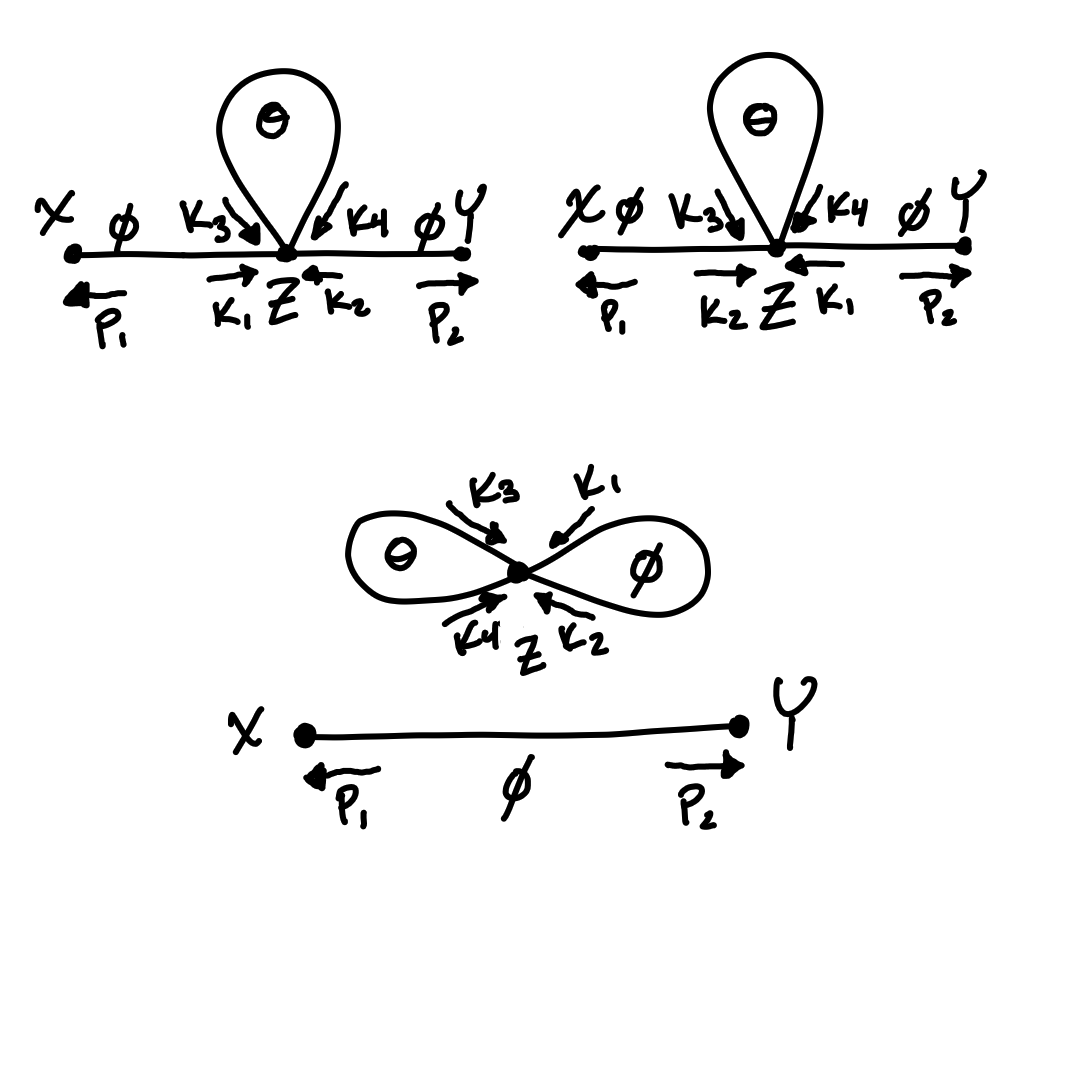
\includegraphics[width=0.6\textwidth,trim={0 2cm 0 0},clip]{feynDias.png}
	\caption{Feynman diagrams contributing to ``leading-order'' two-point correlator.}
	\label{fig:twoPtFeyn}
\end{figure}

Although one can argue that the zero-order pieces are the leading-order contributions, it tends to make a bit more sense to count the number of couplings included in the 
computation, so we will use ``leading order'' to mean ``single-coupling insertion.'' Then, in momentum space, the leading-order two-point function for $\phi$ is given by
\begin{equation}\begin{split}
    \Pi^{(1)}_\phi(X, Y) =& -\frac{i\lambda_{\phi\theta}}{4}\int \mathcal{D}\phi\mathcal{D}\theta\,\int\frac{d^2P_1}{(2\pi)^2}\int\frac{d^2 P_2}{(2\pi)^2}\td\phi(P_1)\td\phi(P_2)
	e^{-iX\cdot P_1}e^{-iY\cdot P_2} \times\\[0.5em]
    &\times \int\Bigg(\prod_{n=1}^4\frac{d^2K_n}{(2\pi)^2}\Bigg)\td{\phi}(K_1)\td\phi(K_2)\td\theta(K_3)\td\theta(K_4)(2\pi)^2\delta^{(2)}(K_1+K_2+K_3+K_4)\,e^{i(S_0 + i\epsilon\text{ terms})}\,.
\end{split}\end{equation}
Now, we simply use our rules for Gaussian integration and sum over all possible ways of connecting similar fields with the free momentum-space propagator, Eq.~\eqref{eq:momProp}. 
Unfortunately, this is a combintorical problem, so the number of contractions grows quite fast. Luckily, in this case, we only get three terms
\begin{equation}\begin{split}\label{eq:LOtwopointexp}
    \Pi_\phi^{(1)}(X, Y) &= -\frac{i\lambda_{\phi\theta}}{4}\int\frac{d^2P_1}{(2\pi)^2}\frac{d^2P_2}{(2\pi)^2}\Bigg(\prod_{n=1}^4\frac{d^2K_n}{(2\pi)^2}\Bigg)\,
	\frac{i(2\pi)^2\delta^{(2)}(K_3 + K_4)}{K_3^2 - m_\theta^2 + i\epsilon}\Bigg[\\[0.5em]
    &\frac{i(2\pi)^2\delta^{(2)}(K_1 + P_1)\,i(2\pi)^2\delta^{(2)}(K_2 + P_2)}{(K_1^2 - m_\phi^2 + i\epsilon)(K_2^2 - m_\phi^2 + i\epsilon)} 
	+ \frac{i(2\pi)^2\delta^{(2)}(K_1 + P_2)\,i(2\pi)^2\delta^{(2)}(K_2 + P_1)}{(K_1^2 - m_\phi^2 + i\epsilon)(K_2^2 - m_\phi^2 + i\epsilon)} \\[0.5em]
    &+\frac{i(2\pi)^2\delta^{(2)}(K_1 + K_2)\,i(2\pi)^2\delta^{(2)}(P_1 + P_2)}{(K_1^2 - m_\phi^2 + i\epsilon)(P_1^2 - m_\phi^2 + i\epsilon)}\Bigg](2\pi)^2
	\delta^{(2)}(K_1 + K_2 + K_3 + K_4)e^{-i(P_1\cdot X + P_2\cdot Y)}\,.
\end{split}\end{equation}
From this expression, we can see that it is possible to represent each of these terms with a diagram: we have fixed points at $X$ and $Y$ representing our external states, 
and a single internal vertex at some other point (call it $Z$) coming from the insertion of the interaction term. We then connect the lines from the vertex in all possible ways 
with corresponding lines (either from the external points or from other lines on the vertex itself). We can get the corresponding mathematical expression by replacing the 
vertex with $-i\lambda_{\phi\theta}/4(2\pi)^2\delta^{(2)}(K_1 + K_2 + K_3 + K_4)$, and each line with the free two-point function. Finally, we integrate over all momenta, 
including the extra Fourier exponentials for the external states. This method of generating all of such diagrams is known as the Feynman diagram expansion, and the corresponding 
rules for replacing each part of a diagram with mathematical expressions are known as the Feynman rules. For this
theory, then, the Feynman rules are given by\footnote{Here, in the two-point function, we do not account for an
additional facor of 4 which arises from the symmetry of the external legs, as is usually standard. This is because we
wish to explicitly show how this arises from the pairing of indices in the path integral.}:
\begin{equation}\begin{split}
	&\text{Two-point $(\phi(P_1), \phi(P_2))$}: \qquad \frac{i(2\pi)^2\delta^{(2)}(P_1 + P_2)}{P_1^2 - m_\phi^2 + i\epsilon} \\[0.5em]
	&\text{Two-point $(\theta(P_1), \theta(P_2))$}: \qquad \frac{i(2\pi)^2\delta^{(2)}(P_1 + P_2)}{P_1^2 - m_\phi^2 + i\epsilon} \\[0.5em]
	&\text{Four-point $(\phi(P_1), \phi(P_2), \theta(P_3), \theta(P_4))$}: \qquad
	-\frac{i\lambda_{\theta\phi}}{4}(2\pi)^2\delta^{(2)}(P_1 + P_2 + P_3 + P_4)\,.
\end{split}\end{equation}
The diagrams for the three terms in Eq.~\eqref{eq:LOtwopointexp} are shown in Fig.~\ref{fig:twoPtFeyn}.

Examining Eq.~\eqref{eq:LOtwopointexp}, the second line can be simplified by the fact that the integrals are symmetric under $K_1\leftrightarrow K_2$, so the two terms in the sum are 
actually the same, just giving a factor of two. Collapsing the delta functions, we arrive at the expression for the momentum-space two-point function
\begin{equation}\begin{split}\label{eq:Pi1}
    \td\Pi_\phi^{(1)}(P) = -\frac{\lambda_{\phi\theta}}{P^2 - m_\phi^2+i\epsilon}\Bigg[&\frac{1}{2}\frac{1}{P^2 - m_\phi^2 + i\epsilon}\int\frac{d^2K}{(2\pi)^2}\frac{1}{K^2 - m_\theta^2 + i\epsilon}\\[0.5em]
    &+ \frac{1}{4}\int\frac{d^2K}{(2\pi)^2}\frac{d^2L}{(2\pi)^2}\frac{(2\pi)^2\delta^{(2)}(0)}{(K^2 - m_\theta^2 + i\epsilon)(L^2 - m_\phi^2 +i\epsilon)}\Bigg]\,.
\end{split}\end{equation}
Now, we have a problem: both of these terms are divergent. The second term features a far worse divergence than the first, proportional to $\delta^{(2)}(0)$, but it is also just 
proportional to the zero-order propagator, so we can simply view this as correction to the normalization of our constant vacuum energy, absorb it into $\mathcal{A}$, and ignore it 
entirely (again, remember that the vacuum energy is already a divergent quantity, but we can only really measure changes in energy, in which case this divergent piece will always cancel). 
While this is an important point to understand, and in some contexts can be physically important, these contributions are irrelevant to what we actually want to calculate, so we will 
ignore any diagrams that appear with such disconnected ``vacuum bubbles.''

On the other hand, the first term, we cannot just get rid of and we have to treat with a bit of care because it actually affects the propagation (and other interactions) of the particle. 
We will discuss the treatment of this divergence more in the next section.

\subsubsection{Renormalziation}

The divergence appearing in the first expression of Eq.~\eqref{eq:Pi1} may be extremely disturbing at first glance, but as it turns out, it isn't as problematic as it seems. To see why, 
we need to again make sure we are asking physical questions. As a first taste of this, we will consider rescaling the fields in the theory by some field- and momentum-independent constant 
(the square roots are just convention)
\begin{equation}\label{eq:fieldRen}
    \phi \to Z_\phi^{1/2}\phi, \quad \theta \to Z_\theta^{1/2}\theta\,.
\end{equation}
Does this make any detectable change in the theory? Recall that the integrand of the path integral after doing a perturbative expansion in $S_I$ will always be polynomial times a 
free-particle Gaussian. Then, to perform the integral, we connect any two like fields in the polynomial part with the inverse of the Gaussian operator (what we called $A$ or $\td A$) 
in all possible ways. However, under the rescaling Eq.~\eqref{eq:fieldRen} each pair of fields in the polynomial part will come with a factor of $Z_i$, but the free action is also 
rescaled by a total factor of $Z_i$, since it is quadratic in the fields. This means that $A_i^{-1}\to 1/Z_i\,A^{-1}$ under such a rescaling and the $Z_i$'s cancel in each pair
\footnote{It is important to note that the integration measures also change under such a rescaling, but since we divide by the zero-insertion path integral, the rescaling of the measures 
cancel between the numerator and denominator.}! So, we find that \textit{the overall normalization of the fields is an unphysical parameter}: any rescaling is guaranteed to drop out in 
calculations of correlation functions.

For other free parameters of the theory, like the couplings and the masses, we need to think about how we can actually measure these quantities. For couplings like $\lambda_{\phi\theta}$, 
we can only really measure such parameters by measuring the outcomes of certain experiments, such as $\phi\phi\to\theta\theta$ in this case. However, it is important to remember that, 
whether we like it or not, all orders of the perturbative expansion play out in nature. So, in such an experiment, we are not just measuring the leading-order, single-$S_I$ insertion, 
so we see that the only physical thing we can extract from experiment is the combination of this single insertion (which is proportional to the classical parameter $\lambda_{\phi\theta}$) 
\textit{plus all quantum corrections to the process}. So again, the $\lambda_{\phi\theta}$ that appears in the Lagrangian is not a physical parameter that we can unambiguously extract from experiment.

Finally, we will consider masses, which are perhaps the most concrete example of this. In this case, the physical thing that we can measure is the pole of the propagator, i.e. the mass 
of $\phi$ is when $P^2 = m_\phi^2$ (and similar for $\theta$). However, again, we need to consider the quantum corrections to the free propagator as the particle travels from $X$ to $Y$. 
In particular, we will consider the set of diagrams that cannot be cut along a single line to separate them, known as one-particle irreducible (1PI) diagrams. Then, the 1PI two-point function, 
$\td\Pi_i^{\text{1PI}}(P^2)$ is given by the sum of all such diagrams. We can then connect these 1PI two-point functions with free propagators to get the full two-point function
\begin{equation}\begin{split}
    \td\Pi_i(P^2) =& \frac{i}{P^2 - m_i^2 + i\epsilon} + \frac{i}{P^2-m_i^2 + i\epsilon}\td\Pi_i^{\text{1PI}}(P^2)\frac{i}{P^2-m_i^2 + i\epsilon}\\[0.5em]
    &+ \frac{i}{P^2-m_i^2+ i\epsilon}\td\Pi_i^{\text{1PI}}(P^2)\frac{i}{P^2-m_i^2 + i\epsilon}\td\Pi_i^{\text{1PI}}(P^2)\frac{i}{P^2-m_i^2 + i\epsilon} + \dots\,,
\end{split}\end{equation}
or
\begin{equation}\label{eq:resumProp}
    \td\Pi_i(P^2) = \frac{i}{P^2 - m_i^2 + i\epsilon}\sum_{n=0}^\infty \Bigg(\td\Pi_i^{\text{1PI}}(P^2)\frac{i}{P^2-m_i^2 + i\epsilon}\Bigg)^n =
	\frac{i}{P^2 - m_i^2 - i\td\Pi_i^{\text{1PI}}(P^2) + i\epsilon} \,,
\end{equation}
where in the second step, we used the expression for the summation of a geometric series. From this, it is clear that the only physical thing we can measure is the 
\textit{combination of $m_i^2$ and $\td\Pi_i^\text{1PI}(P^2)$}, which is again, the mass parameter appearing in the Lagrangian plus all additional quantum corrections.

So, we see that if we measure reasonably finite physical quantities (which again, are combinations of the Lagrangian parameters and the quantum corrections in e.g. $\td\Pi_i^{\text{1PI}}$), 
then any divergences that appear in the (unphysical) quantum corrections must cancel corresponding divergences in the (unphysical) Lagrangian parameters to yield a finite physical result. 
We stress that we are only playing around with unphysical quantities; other divergences can arise that have physical interpretations (and in fact, are not problematic at all), that we cannot get rid.

A very nice methodology of book-keeping for all of these divergent quantities in a consistent way is known as \textit{renormalization}. To renormalize the theory, we consider taking all 
of the unphysical parameters which appear in the original Lagrangian (denoted with a ``$(0)$'' superscript) and replace them with new, rescaled quantities
\begin{equation}
    \phi^{(0)}(x) = \sqrt{Z_\phi}\phi(x), \quad \theta^{(0)}(x) = \sqrt{Z_\theta}\theta(x), \quad {m_\phi^{(0)}}{}^2 = Z_{m_\phi}m_\phi^2, 
	\quad {m_\theta^{(0)}}{}^2 = Z_{m_\theta}m_\theta^2, \quad \lambda_{\phi\theta}^{(0)} = Z_\lambda \lambda_{\phi\theta}\,.
\end{equation}
We now take into account the fact that we are doing a perturbative expansion in $\lambda_{\phi\theta}$, and quantum corrections are those that enter at higher orders in 
$\lambda_{\phi\theta}$. Another way of saying this is that the classical and quantum theories (and therefore the corresponding parameters) coincide if we neglect higher-order quantum corrections. 
To encapsulate this, we expand the rescaling factors as
\begin{equation}
    Z_i = 1 + \sum_{n = 1}^\infty \Big(\frac{\lambda_{\phi\theta}}{4\pi}\Big)^n\delta Z_i^{(n)} = 1 + \delta Z_i\,.
\end{equation}
These $\delta Z_i$'s are typically called ``counterterms'' because we choose them exactly to counteract the divergences in the quantum corrections. 
Then, the Lagrangian in  Eq.~\eqref{eq:Lag} is given in terms of the rescaled parameters as
\begin{equation}\label{eq:renLag}
    \begin{split}
        \mathcal{L} =& \frac{1 + \delta Z_\phi}{2}\Big(\partial_\mu\phi\,\partial^\mu\phi - (1 + \delta Z_{m_\phi})m_\phi^2\phi^2\Big) 
	    + \frac{1 + \delta Z_\theta}{2}\Big(\partial_\mu\theta\,\partial^\mu\theta - Z_{m_\theta}m_\theta^2\theta^2\Big) \\[0.5em]
        &\hspace{4cm}- (1 + \delta Z_\phi)(1 + \delta Z_\theta)(1 + \delta Z_\lambda)\frac{\lambda_{\phi\theta}}{4}\,\phi^2\theta^2 \\[0.5em]
        =& \frac{1}{2}\Big(\partial_\mu\phi\,\partial^\mu\phi - m_\phi^2\phi^2\Big) + \frac{1}{2}\Big(\partial_\mu\theta\,\partial^\mu\theta - m_\theta^2\theta^2\Big) 
	    - \frac{\lambda_{\phi\theta}}{4}\phi^2\theta^2\\[0.5em]
        &+\frac{\delta Z_\phi}{2}\partial_\mu\phi\,\partial^\mu\phi - (\delta Z_\phi + \delta Z_{m_\phi} + \delta Z_\phi\delta Z_{m_\phi})\frac{m_\phi^2}{2}\phi^2 
	    + \frac{\delta Z_\theta}{2}\partial_\mu\theta\,\partial^\mu\theta - (\delta Z_\theta + \delta Z_{m_\theta} + \delta Z_\theta\delta Z_{m_\theta})\frac{m_\theta^2}{2}\theta^2 \\[0.5em]
        &- (\delta Z_\phi + \delta Z_\theta + \delta Z_\lambda + \delta Z_\phi \delta Z_\theta + \delta Z_\phi \delta Z_\lambda + \delta Z_\theta \delta Z_\lambda 
	    + \delta Z_\phi \delta Z_\theta\delta Z_\lambda)\frac{\lambda_{\phi\theta}}{4}\phi^2\theta^2\,.
    \end{split}
\end{equation}
The first line of the second equality of Eq.~\eqref{eq:renLag} is just the original Lagrangian with classical parameters replaced with renormalized ones. The other terms we collect into 
a separate piece of the action that we denote $S_{\text{ct}}$, known as the ``counterterm action.'' Now, for the final trick: instead of splitting these into a quadratic piece in fields 
and an interaction piece, we will include \textit{everything with $\delta Z$'s into the interaction piece of the action.} This way, all propagators retain the same form as their unrenormalized 
counterparts, but we add an additional ``counterterm action,'' given in momentum space by
\begin{equation}\begin{split}\label{eq:CTact}
    S_{\text{ct}} =& \int\frac{d^2K_1}{(2\pi)^2}\frac{d^2K_2}{(2\pi)^2}\Bigg(\frac{\delta Z_\phi}{2} K_1^2 
	- (\delta Z_\phi + \delta Z_{m_\phi} + \delta Z_\phi \delta Z_{m_\phi})\frac{m_\phi^2}{2}\Bigg)\td \phi(K_1)\td\phi(K_2)(2\pi)^2\delta^{(2)}(K_1 + K_2) \\[0.5em]
    &+\int\frac{d^2K_1}{(2\pi)^2}\frac{d^2K_2}{(2\pi)^2}\Bigg(\frac{\delta Z_\theta}{2} K_1^2 
	- (\delta Z_\theta + \delta Z_{m_\theta} + \delta Z_\theta \delta Z_{m_\theta})\frac{m_\theta^2}{2}\Bigg)\td\theta(K_1)\td\theta(K_2)(2\pi)^2\delta^{(2)}(K_1 + K_2) \\[0.5em]
    &- \int\Bigg(\prod_{n=1}^4\frac{d^2K_n}{(2\pi)^2}\Bigg)(\delta Z_\phi + \delta Z_\theta + \delta Z_\lambda + \delta Z_\phi \delta Z_\theta 
	+ \delta Z_\phi \delta Z_\lambda + \delta Z_\theta \delta Z_\lambda + \delta Z_\phi \delta Z_\theta\delta Z_\lambda)\times\\[0.5em]
    &\hspace{3cm}\times\frac{\lambda_{\phi\theta}}{4}\td\phi(K_1)\td\phi(K_2)\td\theta(K_3)\td\theta(K_4)(2\pi)^2\delta^{(2)}(K_1 + K_2 + K_3 + K_4)\,.
\end{split}\end{equation}
This looks quite terrible, but remember that each counterterm we can treat as a perturbative expansion, so most of the terms won't be relevant until higher orders anyway. Moreover, 
the counterterms must be momentum-independent (otherwise, we add derivatives to the terms in the action, and spoil the cancellations we need), so we can just treat these as constants, 
and they don't actually add much more difficulty to the computation.

A key thing to note: if our theory is to be finite, the only unphysical (called ultraviolet for reasons we will discuss) divergences we run into should be able to be absorbed into these 
five counterterms. This means that we must fix each one with \textit{a single process}, and once fixed, \textit{all other ultraviolet divergences at that order in 
perturbation theory must cancel when including these counterterm interactions.} 
Typically, for simplicity, we choose to fix the counterterms using the $n$-point correlation functions that have the same field content as the term in 
the action, i.e. we fix $\delta Z_\phi$ and $\delta Z_{m_\phi}$ from the two-$\phi$ function, $\delta Z_\theta$ and $\delta Z_{m_\theta}$ from the two-$\theta$ function, 
and $\delta Z_\lambda$ from the four-point $\phi^2\theta^2$ function.

The next thing we need to address is the fact that there is a certain amount of arbitrariness to how we choose these counterterms. Consider we break up the amplitude that 
we are calculating into a piece that depends on counterterms, $\mathcal{A}_{\text{ct}}$ and a piece which does not, $\mathcal{A}_{\text{bare}}$. Both of these parts of the amplitude 
will be momentum-dependent in general, so we must require that
\begin{equation}
    \mathcal{A}_{\text{total}}(P_\ell) = \mathcal{A}_{\text{ct}}(\delta Z_\ell, P_\ell) + \mathcal{A}_{\text{bare}}(P_\ell) = \text{UV finite}\,.
\end{equation}
We can notice a couple of things about this. Recall that the counterterms cannot be momentum-dependent. Therefore, the momentum-dependence of the divergent pieces of 
$\mathcal{A}_{\text{ct}}$ and $\mathcal{A}_{\text{bare}}$ must be the same in order for us to define the divergent part of $\delta Z_\ell$ in a momentum-independent way. On the other 
hand, since the only requirement is that the final result is UV-finite, we are always free to add or subtract finite contributions from our counterterms; nothing fixes this contribution. 
In other words, we are always free to take finite pieces of $\mathcal{A}_{\text{bare}}$ and absorb them into $\mathcal{A}_{\text{ct}}$.

However, since the finite pieces of the sub-amplitudes are not fixed, there is no guarantee that the momentum-dependences of the \textit{finite} parts of the two pieces of the total amplitude 
are the same. So, when we include some finite subtractions, we must define a particular value of the momentum that we do this rearranging at, known as the \textit{subtraction point}. 
The way we do the subtractions (i.e. the finite pieces we absorb into the counterterms at the subtraction point) is known as the \textit{renormalization scheme}.

One final thing before doing an actual calculation: in order to actually isolate the divergences in the integrals, we will need to regulate the integrals first, i.e. render them finite in a 
way where we can obtain the original result in some limit. Now, it turns out that whenever we do this, we will need to introduce some additional parameters which don't exist in the 
original theory. Of course, the way we choose to regulate the integral is not unique, so the physical results cannot depend on these parameters. Consider an unphysical parameter $\mu$ 
that we absorb into our counterterms. Then, since $Z = Z(\mu)$, we must cancel this contribution in the corresponding renormalized parameter so that the original, bare parameter 
(the one that shows up in our classical theory) does not depend on this parameter. We can concisely describe this in the so-called \textit{renormalization group equations} (RGEs), which in 
a condensed way say that, if we have a bare parameter, $g^{(0)} = f(\mu) Z_g(\mu) g(\mu)$, then we must require (the logarithmic derivative is not necessary, but it will be convenient later)
\footnote{The additional function $f(\mu)$ is not strictly necessary and can be absorbed into $Z_g$, but as we have already defined the rescaling parameters to be expansions around one, 
this definition is more suited for future computations.}
\begin{equation}
    \frac{d g^{(0)}}{d\log\mu} = \frac{df}{d\log\mu}Z_g(\mu)\,g(\mu) + f(\mu)\frac{dZ_g}{d\log\mu}\,g(\mu) + f(\mu) Z_g(\mu)\frac{dg}{d\log\mu} = 0\,,
\end{equation}
or
\begin{equation}\label{eq:RGE}
    \frac{dg}{d\log\mu} = -\frac{g(\mu)}{f(\mu)}\frac{df}{d\log\mu} - \frac{g(\mu)}{Z_g(\mu)}\frac{dZ_g}{d\log\mu}\,.
\end{equation}
Eq.~\eqref{eq:RGE} turns out to be critical for book-keeping: it is easy to lose track of the parametric dependence on $\mu$ in the computation, but the RGEs allow us to keep track 
of this in a very convenient way.

Again, this all may seem a bit sketchy, but remember that neither the sum of ``bare'' diagrams nor the Lagrangian parameters are physical; only their
combination is physical. Furthermore, we know that any physical result \textit{must} be UV-finite, so if the sum of bare diagrams is UV-divergent, the
Lagrangian parameters must also be UV-divergent in exactly the oppostie way.

Another way to think about this is that the divergences of the bare diagrams is telling us that we made a stupid assumption somewhere. Of course, it
is easy to see where this assumption is: we assumed that as $T\to\pm\infty$, the theory coincides exactly with the free theory. However, as we see
here, the particle \textit{interacts with itself}, and so these interactions can never truly be switched off. We have to take this into account by
adjusting the Lagrangian parameters from those in the classical theory that we tried to quantize. In this case, the deep-UV interactions are the most relevant,
which result in divergent corrections to the parameters, but these divergences are exactly the divergences we get from the diagrams using the
unrenormalized parameters. The net result is a finite physical result.


\subsection{Back to the Two-Point Function}

With all of this out of the way, we can now consider adding the terms in Eq.~\eqref{eq:CTact} to our perturbative expansion of the path integral. Keeping only the terms 
$\mathcal{O}(\lambda_{\phi\theta})$, it is straightforward to find that the total two-point function (neglecting the vacuum bubbles) is given by
\begin{equation}
    \tilde{\Pi}^{(1)}_\phi(P^2) = -\frac{\lambda_{\phi\theta}}{(P^2 - m_\phi^2 + i\epsilon)^2}\Bigg[\frac{i}{4\pi}\delta Z_\phi^{(1)}\, P^2 
	- \frac{i}{4\pi}\Big(\delta Z_\phi^{(1)} + \delta Z_{m_\phi}^{(1)}\Big)\,m_\phi^2 + \frac{1}{2}\int\frac{d^2K}{(2\pi)^2}\frac{1}{K^2 - m_\theta^2 + i\epsilon}\Bigg]\,.
\end{equation}
As we know, the integral, which we will call $\mathcal{I}_0(m_\theta^2)$, is divergent, so it will first be helpful to isolate where the problem is. To do this, we will 
first explicitly write this as the integral over two spacetime dimensions
\begin{equation}\begin{split}
    \mathcal{I}_0(m_\theta^2) &= \int_{-\infty}^\infty\frac{dk^0}{2\pi}\int_{-\infty}^\infty\frac{dk}{2\pi}\frac{1}{(k^0)^2 - k^2 - m_\theta^2 + i\epsilon} \\[0.5em]
    &= \int_{-\infty}^\infty\frac{dk^0}{2\pi}\int_{-\infty}^\infty\frac{dk}{2\pi}\frac{1}{(k^0 + \sqrt{k^2 + m_\theta^2} - i\epsilon)(k^0 - \sqrt{k^2 + m_\theta^2}+i\epsilon)}\,.
\end{split}\end{equation}
Now, we will employ a particularly strange trick: notice that, in the integral over $k^0$, we have two poles in the complex-$k^0$ plane: one above the real axis at negaive-valued 
$k^0$ and one below the real axis for positive-valued $k^0$. This means that, if we rotate our integration contour by 90 degrees counterclockwise, we will not need to pass through any poles. 
This is a form of analytic continuation, known as a Wick rotation, and it has a rigorous mathematical backing (though it isn't always guaranteed to work), but to not distract from the actual point, we will 
not go further into this and simply take it as something that does, in fact, work. So, we rotate our integral $k^0\to ik^0_E$ to find
\begin{equation}
    \mathcal{I}_0(m_\theta^2) = -i\int_{-\infty}^\infty\frac{dk_E^0}{2\pi}\int_{-\infty}^\infty\frac{dk}{2\pi}\frac{1}{(k^0_E)^2 + k^2 + m_\theta^2 - i\epsilon}\,.
\end{equation}
Now, we will choose instead to work in polar coordinates where $k_E^0 = K\sin\phi$ and $k = K\cos\phi$
\begin{equation}\label{eq:tadpole}
    \mathcal{I}_0(m_\theta^2) = -i\int_{0}^\infty\frac{dK}{2\pi}\int_0^{2\pi}\frac{d\phi}{2\pi}\frac{K}{K^2 + m_\theta^2}\,,
\end{equation}
where we took the limit as $\epsilon\to 0$ since we no longer need to worry about the poles appearing on our axis of integration. Here, it is easy to identify the problem: 
consider the region of the integral where $K$ is large. In this region, the $K^2$ piece of the denominator dominates and we find
\begin{equation}
    \int^\infty \frac{dK\,K}{K^2 + m_\theta^2} \sim \int^\infty \frac{dK}{K}\sim \lim_{K\to \infty}\log K\,.
\end{equation}
So, the fact that the internal momentum of the Feynman diagram is allowed to go to infinity is what results in the divergence. This source of divergence is known as an 
\textit{ultraviolet divergence.} There also exist infrared divergences which have a bit of a different resolution, but we won't worry about that for now, since all of our 
integrals in this theory are IR finite.

Now, there are many, many ways that we could regulate this integral to render it finite so that we can extract the divergence. However, one of the nicest in terms of its theoretical 
structure is known as \textit{dimensional regularization}. The basic idea is that integrals of the type~\eqref{eq:tadpole} can actually be neatly solved in an arbitrary number of dimensions. 
To see, this consider
\begin{equation}\label{eq:gendInt}
    \mathcal{I}^{(n)}_d(m^2) = \int\frac{d^dK}{(2\pi)^d}\frac{1}{(K^2 + m^2)^n} = \int\frac{d\Omega_d}{(2\pi)^d}\int_0^\infty\frac{dK\,K^{d-1}}{(K^2 + m^2)^n}\,,
\end{equation}
where in the second step, we chose to use $d$-dimensional spherical coordinates and $d\Omega_d$ is the differential solid angle of a $d-1$ sphere. The integral over this solid angle 
just gives the surface area of this $d-1$-sphere, which has a very nice generalization to $d$-dimensions in terms of the $\Gamma$-function (basically the generalization of the 
factorial to continuous variables)
\begin{equation}
    \int d\Omega_d = \frac{2\pi^{d/2}}{\Gamma\big(\frac{d}{2}\big)}\,.
\end{equation}
Next, we will rescale $K\to m \kappa$ and define the new variable $u = (\kappa^2 + 1)^{-1}$
\begin{equation}
    \mathcal{I}_d(m^2) = \frac{1}{(2\pi)^d}\frac{2\pi^{d/2}}{\Gamma\big(\frac{d}{2}\big)}\,m^{d-2n}\int_0^\infty\frac{d\kappa\,\kappa^{d - 1}}{(\kappa^2 + 1)^n} 
	= \frac{1}{(2\pi)^d}\frac{\pi^{d/2}}{\Gamma\big(\frac{d}{2}\big)}\,m^{d-2n}\int_0^1du\,u^{n-\frac{d}{2}-1}(1-u)^{\frac{d}{2}-1}\,.
\end{equation}
This integral can actually be solved again for general $n$ and $d$ in terms of the Euler Beta Function, which can be written again in terms of $\Gamma$-functions as
\begin{equation}
    \mathcal{I}^{(n)}_d(m^2) = \frac{m^{d-2n}}{(4\pi)^{d/2}}\frac{\Gamma\big(n - \frac{d}{2}\big)\Gamma\big(\frac{d}{2}\big)}{\Gamma\big(\frac{d}{2}\big)\Gamma(n)}\,.
\end{equation}
Now, the source of the poles is readily apparent: the $\Gamma$-function has poles at any integer value $n$ for $n\le 0$. So, in our case, when $n = 1$ and $d = 2$, the numerator 
will diverge! However, the $\Gamma$-function also admits a very nice property that it can be expanded around any one of its poles
\begin{equation}
    \Gamma(\epsilon - n) = \frac{(-1)^n}{n!}\Big(\frac{1}{\epsilon}-\gamma_E + \psi^{(0)}(n + 1) + \frac{\epsilon \pi^2}{6} + \frac{\epsilon}{2}\Big[\psi^{(0)}(n + 1)^2 - \psi^{(1)}(n + 1)\Big] + \mathcal{O}(\epsilon^2)\Big)\,,
\end{equation}
where $\gamma_E \approx 0.5772$ is the Euler constant and $\psi^{(m)}$ is the $m$th Polygamma function. For positive integer $n$, the zeroth Polygamma function is given by
\begin{equation}
    \psi^{(0)}(n + 1) = \sum_{m = 1}^n\frac{1}{n}\,.
\end{equation}

At this point, we are ready for the magic of dimensional regularization: since we are able to evaluate the integrals we need analytically in any number of spacetime dimensions, 
we will continue our spacetime away from $d =2$ and instead work in $d = 2-2\epsilon$ dimensions. Then, once we have renormalized the theory and obtain a finite result, we can 
take $\epsilon\to 0$ and recover the original theory. However, we need to be a bit careful with dimensions. When we take our two-dimensional integrals and upgrade them to $d$-dimensions, 
the mass-dimensions of the problem will no longer work out. In particular, in two dimensions, the integral $\mathcal{I}_0(m_\theta^2)$ is dimensionless, but if we naively continue it to $d$-dimensions, 
it will have mass dimension $d-2 = -2\epsilon$. So, to compensate, we will introduce an artificial mass parameter $\mu$ and take
\begin{equation}
    \int\frac{d^2K}{(2\pi)^2} \to \Big(\frac{\bar \mu}{4\pi}e^{\gamma_E}\Big)^{2\epsilon}\int\frac{d^dK}{(2\pi)^d} = \mu^{2\epsilon}\int\frac{d^dK}{(2\pi)^d}\,,
\end{equation}
where the weird factors in the middle step are chosen to cancel corresponding factors that appear in the expansion of the other parts of the integral. More properly, we should 
view this as the coupling constant $\lambda_{\phi\theta}$ picking up an additional mass dimension which we cancel off by redefining
$\lambda_{\phi\theta}\to \mu^{2\epsilon}\lambda_{\phi\theta}$.

With all of this together, we can finally evaluate our integral
\begin{equation}
    \mathcal{I}_0(m_\theta^2) = -\frac{i}{(4\pi)^{1 - \epsilon}}\Big(\frac{\mu^2}{m_\theta^2}\Big)^\epsilon\Gamma(\epsilon) = -\frac{i}{4\pi}\Big(\frac{1}{\epsilon} 
	+ \log\frac{\bar{\mu}^2}{m_\theta^2}\Big) + \mathcal{O}(\epsilon)\,,
\end{equation}
where we discard all terms order $\epsilon$ and higher because we want to take the limit as $\epsilon\to 0$ once the result is finite. Using this, we find
\begin{equation}
    \td\Pi^{(1)}_\phi(P^2) = -\frac{i\lambda_{\phi\theta}}{4\pi}\frac{1}{(P^2 - m_\phi^2 + i\epsilon)^2}\Bigg[\delta Z_\phi^{(1)}\,P^2 - \Big(\delta Z_\phi^{(1)} 
	+ \delta Z_{m_\phi}^{(1)}\Big)m_\phi^2 - \frac{1}{2\epsilon} - \frac{1}{2}\log\frac{\bar\mu^2}{m_\theta^2}\Bigg]\,.
\end{equation}
As we already stated, the divergent parts of the counterterms are entirely determined by matching the momentum-dependence of the poles since these divergences must cancel for 
all choices of momenta. Since the pole here is momentum-independent, $\delta Z_\phi^{(1,\text{div})} = 0$ and therefore
\begin{equation}
    \delta Z_{m_\phi}^{(1,\text{div})} = -\frac{1}{\epsilon}\frac{1}{2m_\phi^2}\,.
\end{equation}
The inverse mass dependence is to be expected since $Z_{m_\phi}$ is dimensionless, but $\lambda_{\phi\theta}$ has mass dimension two.

Finally, we need to fix our renormalization scheme. Of course, the simplest choice is to just wash our hands, be done and not absorb any more factors into the counterterms. 
This is known as the \textit{minimal subtraction (MS)} (or $\overline{\text{MS}}$ since we use $\bar\mu$ instead of $\mu$) scheme. However, we can make the mass parameters 
a bit more physical if we require that the poles in the propagators (which if we recall, are the true, physical masses of the particles) coincide with $m_\phi^2$. In other words, 
we want to require that, when $P^2 = m_\phi^2$, the denominator of Eq.~\eqref{eq:resumProp} vanishes (up to $i\epsilon$ pieces). This clearly means that we should require 
$\td\Pi_\phi(m_\phi^2) = 0$. With this, we choose our counterterms
\begin{equation}
    \delta Z_\phi^{(1)} = 0, \qquad \delta Z_{m_\phi} = -\frac{1}{2m_\phi^2}\Bigg(\frac{1}{\epsilon} + \log\frac{\bar\mu^2}{m_\theta^2}\Bigg)\,.
\end{equation}
This choice ensures that $m_\phi^2$ (and $m_\theta^2$) are the fixed parameters measured by experiment and therefore do not run via the RGEs. This is known as the \textit{on-shell (OS)} scheme. 
Conveniently, we see that for this choice of renormalization scheme, the leading-order correction to the two-point correlator exactly vanishes for all momenta, $\td\Pi_\phi^{(1)}(P^2) = 0$! 
Of course, the story is the same for $\theta$ with masses swapped, and so
\begin{equation}
    \delta Z_\theta^{(1)} = 0\,, \qquad \delta Z_{m_\theta} = -\frac{1}{2m_\theta^2}\Bigg(\frac{1}{\epsilon} + \log\frac{\bar{\mu}^2}{m_\phi^2}\Bigg)\,, \qquad \td{\Pi}_\theta^{(1)}(P^2) = 0\,.
\end{equation}

\subsection{Two-to-two Scattering}

With all of this in hand, we are now finally ready to tackle a true interacting process. The setup will be as follows: we will start with two $\phi$ particles at spacetime positions 
$X_1^\mu = (0, x_1)$ and $X_2^\mu = (0, x_2)$, with some spread determined by position-space distribution
\begin{equation}
    f(x-x') = \int\frac{dp}{2\pi}\td f(p - p') e^{ip(x-x')}\,,
\end{equation}
where we defined the corresponding momentum-space distribution since it will usually be easier to numerically evaluate the momentum-space integrals than the position-space ones. 
Then, after some time $t$, we will probe the system for a certain number of final state particles: $\{\phi(Y_1),\phi(Y_2)\}$ and $\{\theta(Y_1),\theta(Y_2)\}$. 
We can immediately see that we need an even number of the same particle flavor in the final state since we have two $\phi$'s in the initial state, and 
our action has a $\mathbb{Z}_2$ symmetry under $\phi\to-\phi$ and/or $\theta\to-\theta$, so we can't start with two $\phi$'s and end up with a final
state like $\{\phi(Y_1),\theta(Y_2)\}$. Finally, we want just a probability to measure a single particle, without knowledge of other 
particles in the system, so we will integrate over $y_2$ to only get a distribution in terms of $y_1$ at time $t$.

\subsubsection{Zeroth Order}

To begin, we will consider the simplest (and indeed trivial) case of $\phi\phi\to\phi\phi$ at zeroth order. This is computed with
\begin{equation}\begin{split}\label{eq:trivFourpt}
    \int& dx_1'dx_2' f(x_1-x_1')f(x_2 - x_2')\mel{\Omega}{\phi(Y_2)\phi(Y_1)\phi(X_2')\phi(X_1')}{\Omega}^{(0)}\\[0.5em]
    &= \mathcal{A}\int\mathcal{D}\phi\mathcal{D}\theta\int\Bigg(\prod_{i=1}^4\frac{d^2P_i}{(2\pi)^2}\Bigg)\td f(p_1-p'_1)\td f(p_2-p'_2)\td\phi(P_1)\td\phi(P_2)\td\phi(P_3)\td\phi(P_4)
	e^{-i(P_1\cdot X_1+P_2\cdot X_2 + P_3\cdot Y_2 + P_4\cdot Y_2)}e^{i(S_0+i\epsilon\text{ terms})}\\[0.5em]
    &=\int\Bigg(\prod_{i=1}^4\frac{d^2P_i}{(2\pi)^2}\Bigg)\td f(p_1-p'_1)\td f(p_2-p'_2)\Big(\pi_\phi(P_1,P_2)\pi_\phi(P_3,P_4)\\[0.5em]
    &\hspace{2cm}+ \pi_\phi(P_1,P_3)\pi_\phi(P_2,P_4) + \pi_\phi(P_1,P_4)\pi_\phi(P_2,P_3)\Big)e^{-i(P_1\cdot X_1 + P_2\cdot X_2 + P_3\cdot Y_1 + P_4\cdot Y_2)}\,,
\end{split}\end{equation}
where we defined the momentum-space propagator
\begin{equation}
    \pi_i(P_1, P_2) \equiv \frac{i(2\pi)^2\delta^{(2)}(P_1 + P_2)}{P_1^2 - m_i^2 + i\epsilon}\,.
\end{equation}
Notice that the first product in Eq.~\eqref{eq:trivFourpt} connects causally disconnected points: it pairs the particles at $X_1$ and $X_2$ as well as those at 
$Y_1$ and $Y_2$. Although this will give a non-zero result, it is a pure correlation and not really relevant to the question we are asking, so we will neglect it 
(otherwise, we would have to consider an infinite number of $n$-point functions that account for all pure correlations). This will be exponentially suppressed anyway, so 
neglecting these contributions will not make a big impact on the result.

Of course, the remaining two pieces of Eq.~\eqref{eq:trivFourpt} are just products of two two-point functions. So our leading-order four-point function for $\phi\phi\to\phi\phi$ scattering is just
\begin{equation}\begin{split}
    \Lambda^{(0)}_{\phi\phi}(X_1, X_2, Y_1, Y_2) =& \int\frac{d^2P_1}{(2\pi)^2}\frac{i \td f(p_1-p'_1) e^{-i P_1\cdot (Y_1 - X_1)}}{P_1^2 - m_\phi^2 + i\epsilon}
	\int\frac{d^2P_2}{(2\pi)^2}\frac{i \td f(p_2-p'_2) e^{-i P_2\cdot (Y_2 - X_2)}}{P_2^2 - m_\phi^2 + i\epsilon} \\[0.5em]
    &+\int\frac{d^2P_1}{(2\pi)^2}\frac{i \td f(p_1-p'_1) e^{-i P_1\cdot (Y_2 - X_1)}}{P_1^2 - m_\phi^2 + i\epsilon}\int\frac{d^2P_2}{(2\pi)^2}\frac{i \td f(p_2-p'_2) 
	e^{-i P_2\cdot (Y_1 - X_2)}}{P_2^2 - m_\phi^2 + i\epsilon}\,.
\end{split}\end{equation}

Of course, if we insert any $\theta$'s, we will simply get zero (aside from correlations) since $\phi$ cannot turn into a $\theta$ simply by propagation; it needs interactions to do so!

\subsubsection{First Order}

The story becomes a bit more interesting at leading order in $\lambda_{\phi\theta}$. However, the first process we consider is again a trivial (albeit necessary) one; we will 
again consider the $\phi\phi \to \phi\phi$ case to linear order in the interactions. Recalling that we also need to insert $\delta Z_{m_i}^{(1)}$ since it is linear in 
$\lambda_{\phi \theta}$ (we do not need to include any factors of $\delta Z_\lambda^{(1)}$ since this part of the action begins at $\mathcal{O}(\lambda_{\phi\theta}^2)$ due to the 
additional factor of the coupling in the bare term), neglecting pure correlations and vacuum bubbles, and skipping a couple of steps, we find
\begin{equation}\begin{split}\label{eq:FOphiphi}
    &\Lambda_{\phi\phi}^{(1)}(X_1, X_2, Y_1, Y_2) = -i\lambda_{\phi\theta}\int\Bigg(\prod_{n=1}^4\frac{d^2P_n}{(2\pi)^2}\Bigg)\td f_1\td f_2 
	e^{-i(P_1\cdot X_1 +P_2\cdot X_2 + P_3\cdot Y_1 + P_4\cdot Y_2)}\Bigg[\\[0.5em]
    &2\times\frac{1}{4}\int\Bigg(\prod_{m = 1}^4\frac{d^2 K_m}{(2\pi)^2}\Bigg)\pi_\theta(K_3, K_4)\Bigg\{\pi_\phi(K_1,P_1)\pi_\phi(K_2,P_3)\pi_\phi(P_2,P_4) 
	+ \pi_\phi(K_1,P_1)\pi_\phi(K_2,P_4)\pi_\phi(P_2,P_3) \\[0.5em]
    &\hspace{1cm} + \pi_\phi(K_1,P_2)\pi_\phi(K_2,P_3)\pi_\phi(P_1,P_4) + \pi_\phi(K_1,P_2)\pi_\phi(K_2,P_4)\pi_\phi(P_1,P_3)\Bigg\}(2\pi)^2\delta^{(2)}(K_1 + K_2 + K_3 + K_4)\\[0.5em]
    &+2\times\frac{\delta Z_{m_\phi} m_\phi^2}{2}\int\Bigg(\prod_{m = 1}^2\frac{d^2 K_m}{(2\pi)^2}\Bigg)\Bigg\{\pi_\phi(K_1,P_1)\pi_\phi(K_2,P_3)\pi_\phi(P_2,P_4) 
	+ \pi_\phi(K_1,P_1)\pi_\phi(K_2,P_4)\pi_\phi(P_2,P_3) \\[0.5em]
    &\hspace{1cm} + \pi_\phi(K_1,P_2)\pi_\phi(K_2,P_3)\pi_\phi(P_1,P_4) + \pi_\phi(K_1,P_2)\pi_\phi(K_2,P_4)\pi_\phi(P_1,P_3)\Bigg\}(2\pi)^2\delta^{(2)}(K_1 + K_2)\Bigg]\,.
\end{split}\end{equation}
The factors of two that we kept explicit are coming from replacing $K_1\leftrightarrow K_2$ in the integrals and getting the same overall factor. 
This is to essentially keep in mind that each diagram that we draw comes with a ``symmetry factor'' that we have to account for in order to count repeated diagrams.

Eq.~\eqref{eq:FOphiphi} looks very obscure, but when we represent it in the language of Feynman diagrams, it is clear what is happening: we are simply computing the corrected propagation 
between each of the points from the first-order two-point functions! However, if we choose the on-shell renormalization scheme, we saw that, since the $\theta$ loops do not 
feature an explicit dependence on momentum, the first order two-point function exactly vanishes. So, we have the very nice result
\begin{equation}
    \Lambda_{\phi\phi}^{(1)}(X_1, X_2, Y_1, Y_2) = 0\,.
\end{equation}
Note that, in another renormalization scheme, such as $\overline{\text{MS}}$, this would not be the case. However, in this scheme, the masses would be running parameters, and 
would pick up a $\log\bar{\mu}$-dependence, which would cancel between the zeroth order (the propagators would depend on $m_\phi(\bar{\mu})$) and this
leading-order result (see the Appendix for an explicit calculation). 

Next, we need to find an expression for $\phi\phi\to\theta\theta$ at this order. This expression turns out to be a bit simpler once we neglect correlations and bubbles:
\begin{equation}\begin{split}
    &\Lambda_{\theta\theta}(X_1, X_2, Y_1, Y_2) = -i\frac{\lambda_{\phi\theta}}{4}\int\Bigg(\prod_{n=1}^4\frac{d^2P_n}{(2\pi)^2}\Bigg)\td f_1\td f_2 
	e^{-i(P_1\cdot X_1 +P_2\cdot X_2 + P_3\cdot Y_1 + P_4\cdot Y_2)}\Bigg[\\[0.5em]
    &4\times\int\Bigg(\prod_{m=1}^4\frac{d^2K_m}{(2\pi)^2}\Bigg)\,\pi_\phi(K_1, P_1)\pi_\phi(K_2, P_2)\pi_\theta(K_3, P_3)\pi_\theta(K_4, P_4)(2\pi)^2\delta^{(2)}(K_1 + K_2 + K_3 + K_4)\Bigg]\,,
\end{split}\end{equation}
where again, the symmetry factor arises due to the fact that there are two ways of connecting $\phi$'s and two ways of connecting $\theta$'s that give the same 
integral under renaming of integration variables. The $K_i$ integrals can all be easily evaluated using the delta functions in $\pi_i$ to give
\begin{equation}\begin{split}\label{eq:fourptLam}
    &\Lambda_{\theta\theta}^{(0)}(X_1, X_2, Y_1, Y_2) =\\[0.5em]
    &-i\lambda_{\phi\theta}\int\Bigg(\prod_{n=1}^4\frac{d^2P_n}{(2\pi)^2}\Bigg)\Bigg[\frac{i\td f_1e^{-iP_1\cdot X_1}}{P_1^2 - m_\phi^2 + i\epsilon
	}\frac{i\td f_2e^{-iP_2\cdot X_2}}{P_2^2 - m_\phi^2 + i\epsilon}\frac{ie^{-iP_3\cdot Y_1}}{P_3^2 - m_\theta^2 + i\epsilon}\frac{ie^{-iP_4\cdot Y_2}}{P_4^2 - m_\theta^2 + i\epsilon}\Bigg]
	(2\pi)^2\delta^{(2)}(P_1 + P_2 + P_3 + P_4)\,.
\end{split}\end{equation}
This integral is much more challenging than the previous ones we considered, and it only gets worse from here! 

One can try to evaluate Eq.~\eqref{eq:fourptLam} directly using e.g. the residue theorem, but after collapsing the delta function and integrating over
all the $P_i^0$'s, one finds non-analytic poles in the remaining integration variables which one cannot evaluate using the residue theorem. The other
problem is that the integral is highly oscillatory, making numerical evaluation (even after using an e.g. Feynman reparameterization) extremely
difficult. In particular, since this is a high-dimensional integral, one would want to use Monte-Carlo integration techniques, but this will not
converge with such a rapidly oscillating integrand.

\section{What We Really Should Calculate}

At the end of the day, the sorts of calculations shown in the last section are not what we do in particle physics; this is partly because the analytical integrals that
we saw are very intractable to actually compute, especially when one goes beyond leading order. They are highly oscillatory integrals with non-trivial pole structures,
which makes them very difficult to compute either analytically or even numerically. However, the question that we asked is still not really aligned with what is studied
in an experiment. Typically, an experimentalst will not delicately prepare two single particles in a particular momentum/position distribution and measure a small number
of particles that comes out. Instead, usually beams of many particles are accelerated and focused into a particular area to interact with each other at a very small
interaction point. Then, once the particles have interacted, they are seen in detectors far from the interaction point.

\subsection{The $S$-Matrix}

This story is reminiscent of what we used to derive the path integral: when we start the particles very far from each other and wait until they are far away from each other
after interacting, the two sets of particles behave like the free-field particles (aside from self-interaction effects, which are accounted for via renormalization). We can
therefore simply consider ``in'' and ``out'' states which are sufficiently non-interacting so that we can treat them as living at times $T\to \pm \infty$. We then define
the elements of the \textit{$S$-matrix}
\begin{equation}
	S_{\alpha\beta} = \braket{\beta,\text{out}}{\alpha,\text{in}}\,.
\end{equation}
The indices $\alpha$ and $\beta$ are really short-hand for a tensor product of all single-particle states that live in the initial and final systems. The $S$-matrix will
give, in general, two contributions: the interacting piece and the non-interacting piece. The latter will simply be given by a delta function between states $\alpha$ and $\beta$,
while the former will give the interesting matrix elements, $M_{\beta \alpha}$. Since this is a Lorentz-invariant theory, we can then write
\begin{equation}
	S_{\alpha\beta} = \delta(\alpha - \beta) + (2\pi)^d i\delta^{(d)}(P_\alpha - P_\beta)M_{\beta \alpha}\,,
\end{equation}
where we assumed we are working in $d$-spacetime dimensions, and the factor of $2\pi i$ is a normalization.

We again emphasize that the states making up the $S$-matrix live in the infinitely distant past and infinitely far future, a good approximation when most interactions
occur at very small length scales. However, we note that the free-field theory will never have bound states in it, so if our interactions do end up producing
bound states which are inseparable even in the limit as $T\to \pm \infty$, the $S$-matrix method will fail\footnote{Interestingly, this happens in
nature with Quantum Chromodynamics (QCD). It turns out that interactions in this theory actually get \textit{stronger} at large separation, so as
$T\to\pm\infty$, particles charged under QCD will always form bound states, called hadrons. This means that one must use a different technique other
than computing $S$-matrix elements to calculate QCD correlation functions.}.

\subsection{LSZ Reduction}

We now wish to get an actual form for the interaction matrix elements, $M_{\beta\alpha}$ in terms of the time-ordered correlation functions that we already know how to compute.
The key assumption is that, after scattering, all of our particles have changed state, even if just by a little. In the language of Feynman diagrams, this corresponds to
the subset of all \textit{connected} Feynman diagrams, simply meaning that we never have any particles propagating directly from the inital to the finial state; they must always
participate in some interactions. This means that no particles that live in $\alpha$ live in $\beta$.
Next, we use the fact that $\Pi(x) = \partial_0\Phi(x)$, as we found from our Legendre transformation to re-write the distant-past creation operator
\begin{equation}
	a^\dag_{\mathbf{p},m;\text{in}} = \lim_{x^0\to-\infty}\int d^{d-1}\mathbf{x}e^{-i(\omega_\mathbf{p} x^0 - \mathbf{p}\cdot\mathbf{x})}
	\Bigg[\sqrt{\frac{\omega_{\mathbf{p}}}{2}}\Phi_m(x) - \frac{i}{\sqrt{2\omega_{\mathbf{p}}}}\partial_0\Phi_m(x)\Bigg]\,,
\end{equation}
where we now represent spacetime vectors as un-bolded letters and spatial vectors as bolded. Introducing the notation $f\overleftrightarrow{\partial_0}g = f\partial_0 g - g\partial_0 f$,
this can be re-written as
\begin{equation}
	a^\dag_{\mathbf{p},m;\text{in}} = \lim_{x^0\to-\infty}\int d^{d-1}\mathbf{x}
	\frac{-i\,e^{-i(\omega_\mathbf{p} x^0 - \mathbf{p}\cdot\mathbf{x})}}{\sqrt{2\omega_{\mathbf{p}}}}\overleftrightarrow{\partial_0}\Phi_m(x)\,.
\end{equation}
Similarly, for the ``out'' annihilation operator, we have
\begin{equation}
	a_{\mathbf{p},m;\text{out}} = \lim_{x^0\to\infty}\int d^{d-1}\mathbf{x}
	\frac{i\,e^{i(\omega_\mathbf{p} x^0 - \mathbf{p}\cdot\mathbf{x})}}{\sqrt{2\omega_{\mathbf{p}}}}\overleftrightarrow{\partial_0}\Phi_m(x)\,.
\end{equation}
It should be noted that, with this definition, the single-particle states have the relativistic normalization $\ket{\mathbf{p}} =
\sqrt{2\omega_{\mathbf{p}}}a^\dag_{\mathbf{p}}\ket{0}$.
Then, by removing one particle from the ``in'' state, our matrix element in question is given by
\begin{equation}
	M_{\beta\alpha} = \sqrt{2\omega_{\mathbf{p}}}\mel{\beta,\text{out}}{a^\dag_{\mathbf{p}_1,m_1;\text{in}}}{\alpha',\text{in}}
	= \sqrt{2\omega_{\mathbf{p}}}\mel{\beta,\text{out}}{a^\dag_{\mathbf{p}_1,m_1;\text{in}}}{\alpha',\text{in}}
	- \sqrt{2\omega_{\mathbf{p}}}\mel{\beta,\text{out}}{a^\dag_{\mathbf{p}_1,m_1;\text{out}}}{\alpha',\text{in}}\,,
\end{equation}
where we used the fact that the $\mathbf{p}_1;m_1$ state doesn't exist in $\beta$, and therefore $\bra{\beta,\text{out}}a^\dag_{\mathbf{p}_1,m_1;\text{out}} = 0$ and the
prime denotes the fact that we have removed a single particle from the in state. Using the explicit expressions for the creation operators, we find
\begin{equation}
	M_{\beta\alpha} = -i\Big(\lim_{x_1^0\to-\infty} - \lim_{x_1^0\to\infty}\Big)\int d^{d-1}\mathbf{x}_1
	e^{-i(\omega_{\mathbf{p}_1}x_1^0 - \mathbf{p_1}\cdot\mathbf{x_1})}\overleftrightarrow{\partial_{x_1^0}}
	\mel{\beta,\text{out}}{\Phi_{m_1}(x_1)}{\alpha',\text{in}}\,.
\end{equation}
By the fundamental theorem of calculus (or the one-dimensional version of Stokes' theorem),
\begin{equation}
	\Big(\lim_{t\to\infty} - \lim_{t\to-\infty}\Big)f(t) = \int_{-\infty}^\infty dt\,\frac{\partial f}{\partial t}\,,
\end{equation}
giving
\begin{equation}\begin{split}
	M_{\beta\alpha} =& i\int\,dx_1^0\partial_{x_1^0}\int d^{d-1}\mathbf{x}_1
	e^{-i(\omega_{\mathbf{p}_1}x_1^0 - \mathbf{p_1}\cdot\mathbf{x_1})}\overleftrightarrow{\partial_{x_1^0}}
	\mel{\beta,\text{out}}{\Phi_{m_1}(x_1)}{\alpha,\text{in}}\\[0.5em]
	=&i\int d^dx_1\Big[e^{-i(\omega_{\mathbf{p}_1}x_1^0 - \mathbf{p}_1\cdot \mathbf{x}_1)}\partial_{x_1^0}^2\mel{\beta,\text{out}}{\Phi_{m_1}(x_1)}{\alpha,\text{in}}
	- \mel{\beta,\text{out}}{\Phi_{m_1}(x_1)}{\alpha,\text{in}}\partial_{x_1^0}^2e^{-i(\omega_{\mathbf{p}_1}x_1^0 - \mathbf{p}_1\cdot \mathbf{x}_1)}\Big]\,.
\end{split}\end{equation}
The complex exponential is just the plane-wave solution to the Klein-Gordon equation, i.e.
\begin{equation}
	(\partial_t^2 - \partial_{\mathbf{x}}\cdot\partial_{\mathbf{x}} + m^2)e^{-i(\omega_{\mathbf{p}}t - \mathbf{p}\cdot \mathbf{x})} = 0\,,
\end{equation}
where $\omega_{\mathbf{p}} = \sqrt{|\mathbf{p}|^2 + m^2}$. Using this and integrating by parts, assuming that the integrand is suitably 
well-behaved\footnote{Really, here we should replace the plane-wave exponential with a well-behaved wave packet that is a linear combination
of plane-waves to guarantee the proper behavior as $|\mathbf{x}|\to\infty$. However, this wave-packet will still be a solution to the Klein-Gordon
equation, so the argument is unchanged.} as $|\mathbf{x}|\to\infty$, we find the matrix element
\begin{equation}
	M_{\beta\alpha} = i\int d^dx_1\,e^{-i\bar{p}_1\cdot x_1}\big(\partial_{x_1,\mu}\partial_{x_1}^\mu + m_{m_1}^2\big)\mel{\beta,\text{out}}{\Phi_{m_1}(x_1)}{\alpha',\text{in}}\,,
\end{equation}
where $\bar{p}^\mu = (\omega_{\mathbf{p}},\mathbf{p})$ is the on-shell $d$-momentum.

Following similar steps, we will now remove a single particle from the ``out'' state, in which case we find the interesting result
\begin{equation}\begin{split}
	&\mel{\beta,\text{out}}{\Phi_{m_1}(x_1)}{\alpha',\text{in}} = 
		\sqrt{2\omega_{\mathbf{k}_1}}\mel{\beta',\text{out}}{a_{\mathbf{k}_1,n_1;\text{out}}\Phi_{m_1}(x_1)}{\alpha',\text{in}}\\[0.5em]
	&=\sqrt{2\omega_{\mathbf{k}_1}}\mel{\beta',\text{out}}{a_{\mathbf{k}_1,n_1;\text{out}}\Phi_{m_1}(x_1)}{\alpha',\text{in}}
		- \sqrt{2\omega_{\mathbf{k}_1}}\mel{\beta',\text{out}}{\Phi_{m_1}(x_1)a_{\mathbf{k}_1,n_1;\text{in}}}{\alpha',\text{in}}\\[0.5em]
	&=i\int d^dy_1e^{i\bar{k}_1\cdot y_1}\big(\partial_{y_1,\mu}\partial^\mu_{y_1} + m_{n_1}^2\big)
		\mel{\beta',\text{out}}{\mathbf{T}\big\{\Phi_{n_1}(y_1)\Phi_{m_1}(x_1)\big\}}{\alpha',\text{in}}\,.
\end{split}\end{equation}
Repeating this process, we find the \textit{Lehmann-Symanzik-Zimmermann (LSZ) reduction formula}
\begin{equation}\begin{split}
	M_{\beta\alpha} = &\prod_{\beta=1}^N\Bigg(i\int\,d^d y_\beta e^{i\bar{k}_\beta\cdot y_\beta}\big(\partial_{y_\beta,\mu}\partial^\mu_{y_\beta} + m_{n_\beta}^2\big)\Bigg)
		\prod_{\alpha=1}^M\Bigg(i\int\,d^d x_\alpha e^{-i\bar{p}_\alpha\cdot x_\alpha}\big(\partial_{x_\alpha,\mu}\partial^\mu_{x_\alpha} + m_{m_\alpha}^2\big)\Bigg)\\[0.5em]
		&\times\mel{\Omega}{\mathbf{T}\big\{\Phi_{n_N}(y_N)\Phi_{n_{N-1}}(y_{N-1})\times\dots\times\Phi_{n_1}(y_1)
			\Phi_{m_1}(x_1)\Phi_{m_2}(x_2)\times\dots\times\Phi_{m_M}(x_M)\big\}}{\Omega}\,.
\end{split}\end{equation}
This formula is even more illuminating if we pass to Fourier variables, defining
\begin{equation}\begin{split}
	&\mel{\Omega}{\mathbf{T}\big\{\Phi_{n_N}(y_N)\times\dots\times\Phi_{n_1}(y_1)\Phi_{m_1}(x_1)\times\dots\times\Phi_{m_M}(x_M)\big\}}{\Omega} =\\[0.5em]
	&\prod_{\beta = 1}^N\Bigg(\int\frac{d^dk_\beta}{(2\pi)^d}e^{ik_\beta\cdot y_\beta}\Bigg)\prod_{\alpha = 1}^N\Bigg(\int\frac{d^dp_\alpha}{(2\pi)^d}e^{ip_\alpha\cdot x_\alpha}\Bigg)
	\Gamma_{m_1,\dots,m_M;n_1,\dots,n_N}\big(p_1,\dots,p_M;k_1,\dots,k_N\big)\,,
\end{split}\end{equation}
where, after shifting the integration variables $k\to -k$, and performing all $x$ and $y$ integrals, we find
\begin{equation}\begin{split}\label{eq:momLSZ}
	M_{\beta\alpha} = \prod_{\beta = 1}^N&\Bigg(-i\int d^d k_\beta \delta^{(d)}(k_\beta - \bar{k}_\beta)\big(k_\beta^2 - m_{n_\beta}^2\big)\Bigg)
		\prod_{\alpha = 1}^N\Bigg(-i\int d^d p_\alpha \delta^{(d)}(p_\alpha - \bar{p}_\alpha)\big(p_\alpha^2 - m_{m_\alpha}^2\big)\Bigg)\\[0.5em]
		&\times \Gamma_{m_1,\dots,m_M;n_1,\dots,n_N}\big(p_1,\dots,p_M;-k_1,\dots,-k_N\big)\,.
\end{split}\end{equation}
This formula is actually quite amazing: it tells us that the interesting part of our $S$-matrix is given exclusively by the residues of the poles in the
momentum-space time-ordered correlation function, setting external momenta on-shell (also note that ingoing versus outgoing momenta are already
taken care of in the formula). This actually makes our lives substantially easier due to the fact that
the big difficulty in calculating correlation functions comes from the complicated pole structure arising from the propagators on each external leg.

One last comment is in order. Even when we let $T\to\pm\infty$, although interactions between particles will be turned off, self-interactions of
a single particle will never disappear. We must therefore not only take into account the renormalization of the fields, but also the fact that
these self-interactions will shift the physical mass. The latter is simple to account for: we simply take $m_i$ in Eq.~\eqref{eq:momLSZ} and
replace it with $m_i^{\text{pole}}$, which is the mass of the particle measured as the pole in the propagator (we already saw that this
accounts for all self-interactions). The former is a bit trickier, but can be accounted for by recognizing that after renormalization, the free one-particle
states are normalized so that
\begin{equation}
	|\mel{\Omega}{\Phi_m(0)}{\lambda_{0,m}}|^2 = Z_m\,,
\end{equation}
where $\ket{\lambda_{0,m}}$ is the zero-momentum, single-particle state with flavor $m$. This immediately implies that the properly normalized states are
then given by
\begin{equation}
	\ket{\mathbf{p};m} = \frac{\sqrt{2\omega_{\mathbf{p};m}}}{\sqrt{Z_m}}a^\dag_{\mathbf{p},m}\ket{\Omega}\,,
\end{equation}
in which case, the renormalized LSZ-reduction formula is given by
\begin{equation}\begin{split}\label{eq:renLSZ}
	M_{\beta\alpha} = \prod_{\beta = 1}^N&\Bigg(-i\int d^d k_\beta \delta^{(d)}(k_\beta - \bar{k}_\beta)\frac{\big(k_\beta^2 - {m^{\text{pole}}_{n_\beta}}^2\big)}{\sqrt{Z_{n_\beta}}}\Bigg)
		\prod_{\alpha = 1}^N\Bigg(-i\int d^d p_\alpha \delta^{(d)}(p_\alpha - \bar{p}_\alpha)\frac{\big(p_\alpha^2 - {m^{\text{pole}}_{m_\alpha}}^2\big)}{\sqrt{Z_{m_\alpha}}}\Bigg)\\[0.5em]
		&\times \Gamma_{m_1,\dots,m_M;n_1,\dots,n_N}^{\text{ren}}\big(p_1,\dots,p_M;-k_1,\dots,-k_N\big)\,.
\end{split}\end{equation}
Qualitatively, this doesn't change much. In fact, Eq.~\eqref{eq:renLSZ} just tells us that the renormalization of the external legs is automatically accounted for when computing
$S$-matrix elements. In other words, we don't need to consider self-energy insertions on external legs, and we can just consider ``amputated'' diagrams where the 
external legs are automatically put on-shell.

\subsection{Scattering Processes}

Now that we know how to actually compute $S$-matrix elements, we should probably figure out how to use them in calculations of physical observables.
We know that the $S$-matrix tells us how probable it is for some initial state $\alpha$ to scatter to final state $\beta$, so the simplest thing that
we can think of is to compute \textit{rates} at which a particular process will occur. To do this, we will pretty much exactly follow the steps of Sec.~3.4
of Weinberg.

We will start by putting the system we care about into a hyper-toroidal ``box'' (i.e. a hyper-cube with all opposite ends identified with each other) with volume $V$, in which case
the momenta of the particles are quantized. Then, the spatial delta functions become
\begin{equation}
	\delta^{(d - 1)}(\mathbf{p}' - \mathbf{p}) \to V\delta_{\mathbf{p}',\mathbf{p}} \equiv \delta_V^{(d-1)}(\mathbf{p}' - \mathbf{p})\,,
\end{equation}
where $\delta_{\mathbf{p}',\mathbf{p}}$ is the ordinary Kronecker delta function. Since we have restricted ourselves to a finite volume, if we allow interactions
to run for an infinite amount of time, all possible interactions will occur an infinite number of times, so we won't get anything meaningful for scattering rates.
In that case, we have to also consider a ``time box'' where we turn on interactions at time $-T/2$ and turn them off at later time $T/2$. In this case, the
energy delta functions are given by
\begin{equation}
	\delta({p'}{}^0 - p^0) \to \frac{1}{2\pi}\int_{-T/2}^{T/2}\,dt\,e^{i({p'}{}^0 - p^0)t} \equiv \delta_T({p'}{}^0 - p^0)\,.
\end{equation}
Recall that in the infinte-volume case, the initial- and final-state wavefunctions are normalized so that
\begin{equation}
	\braket{\Psi_\beta}{\Psi_\alpha} = \delta(\alpha - \beta)\prod_{n=1}^{N_\alpha} 2E_n\,,
\end{equation}
which is just shorthand for saying that if the particles are unchanged between the initial and final state, they should have the same flavors, energies, and momenta.
The additional normalization comes from the standard relativistic normalization of states and $N_\alpha$ is the number of particles in state $\Psi_\alpha$.
However, the spatial momenta delta functions in the box pick up an additional factor of $V$ for each initial/final state particle. Therefore, the initial/final
state wavefunctions pick up an extra factor when put in a box
\begin{equation}
	\ket{\Psi_\alpha} = V^{N_\alpha/2}\prod_{n=1}^{N_\alpha}\sqrt{2E_n}\ket{\Psi^{\text{box}}_\alpha} \quad \Rightarrow \quad 
	\braket{\Psi_\beta^{\text{box}}}{\Psi_\alpha^{\text{box}}} = \delta_{\alpha\beta}\,.
\end{equation}
With this, the ``box'' $S$-matrix is given by
\begin{equation}
	S^{\text{box}}_{\beta\alpha} = \Bigg(\frac{1}{V}\Bigg)^{\frac{N_\alpha + N_\beta}{2}}
	\prod_{m=1}^{N_\alpha}\frac{1}{\sqrt{2E_m}}\prod_{n=1}^{N_\beta}\frac{1}{\sqrt{2E_n}}S_{\beta\alpha}\,.
\end{equation}
This picks out a spicific final state $\beta$ with a single fixed momentum state, but often times, we want to know the transition of
particles with fixed initial momentum state and \textit{any} final momentum state, or we want to know how the transition depends on
the values of the final-state momentum. We therefore need to consider a properly-normalized volume in momentum space, which we will take
to be the small momentum-space box, $d^{d-1}\mathbf{p}/(2\pi)^{d - 1}$ for each particle. Then, the total number of states corresponding to this
momentum-space box will correspond to the combined volume of this momentum-space box and the spatial box, i.e. $Vd^{d-1}\mathbf{p}/(2\pi)^{d-1}$.
Finally, if we do this for all final states of the system, we get a total number of states in this phase-space volume
\begin{equation}
	d\mathcal{N}_\beta = V^{N_\beta}\prod_{n=1}^{N_\beta}\frac{d^{d-1}\mathbf{p}_n}{(2\pi)^{d-1}}\,.
\end{equation}
The probability of measuring a final state within this phase-space volume is given by the probability of transitioning from state $\alpha$ to a state
$\beta$ within this volume, times the total number of states within the volume. The latter is given by $d\mathcal{N}_\beta$, and the former is just
given by $|S_{\beta\alpha}^{\text{box}}|^2$
\begin{equation}
	dP(\alpha\to\beta) = V^{-N_\alpha}|S_{\beta\alpha}|^2\prod_{m=1}^{N_\alpha}\frac{1}{2E_m}\prod_{n = 1}^{N_\beta}\frac{d^{d-1}\mathbf{p}_n}{(2\pi)^{d-1}2E_n}\,.
\end{equation}

Again, we will only really be interested in the case where we have a true interaction, so we will only consider connected matrix elements. Therefore, $\delta(\alpha - \beta) = 0$
and we can use
\begin{equation}
	S_{\beta\alpha} = i(2\pi)^d\delta_T(p_\beta^0 - p_\alpha^0)\delta^{(d-1)}_V(\mathbf{p}_\beta - \mathbf{p}_\alpha)\,M_{\beta\alpha}\,,
\end{equation}
where now that we work in the finite-volume limit, we can take the square of the ``delta functions'' to find
\begin{equation}
	\big(\delta_T(p_\beta^0 - p_\alpha^0)\delta_V^{(d-1)}(\mathbf{p}_\beta - \mathbf{p}_\alpha)\big)^2 \overset{T,V\to\infty}{=}
	\frac{T\,V}{(2\pi)^d}\delta^{(d)}(p_\beta - p_\alpha)\,,
\end{equation}
where we used the fact that, as $T$ and $V$ become very large, the finite delta functions become closer and closer to the true Dirac delta functions. Then, in the
large volume limit, the differential transition probability is given by
\begin{equation}
	dP(\alpha \to \beta) = (2\pi)^d\,T\,V^{1-N_\alpha}\delta^{(d)}(p_\beta - p_\alpha)|M_{\beta\alpha}|^2
	\prod_{m=1}^{N_\alpha}\frac{1}{2E_m}\prod_{n = 1}^{N_\beta}\frac{d^{d-1}\mathbf{p}_n}{(2\pi)^{d-1}2E_n}\,.
\end{equation}
For any system of particles, the differential probability is just proportional to $T$. We can then define the rate to be the probability per unit time
\begin{equation}\label{eq:genRate}
	dR(\alpha\to\beta) = \frac{V^{1-N_\alpha}}{\prod_{m=1}^{N_\alpha}2E_m}|M_{\beta\alpha}|^2d\Phi_{n}(p_\alpha;p_\beta)\,,
\end{equation}
where we defined the $n$-body Lorentz-invariant phase-space factor
\begin{equation}
	d\Phi_n(p_\alpha;p_\beta) = (2\pi)^d\delta^{(d)}(p_\alpha - p_\beta)\prod_{n = 1}^{N_\beta}\frac{d^{d-1}\mathbf{p}_n}{(2\pi)^{d-1}2E_n}\,,
\end{equation}
with the implicit understanding that all external momenta are on-shell, i.e. $E_i = \sqrt{|\mathbf{p}_i|^2 + m_i^2}$. When all is said and done, Eq.~\eqref{eq:genRate}
is really what we are after when we want to make the prediction for the outcome of a particle physics experiment. There are really two very special cases of $N_\alpha = 1$ 
and $N_\alpha = 2$ which are by far the most common to discuss in particle physics contexts.

\subsubsection{Particle Decays ($N_\alpha = 1$)}

In the case where we only have a single particle in the initial state, we are looking at a particle which decays into a set of $N_\beta$ other particles. In this case,
Eq.~\eqref{eq:genRate} reduces to the \textit{differential decay width}
\begin{equation}\label{eq:decayRate}
	d\Gamma((p_0;m_0) \to \beta) = \frac{|M_{\beta\alpha}|^2}{2 E_0}d\Phi(\mathbf{p}_0;\mathbf{p}_\beta)\,.
\end{equation}
This will be simplest to evaluate in the initial-state particle's rest frame, where $E_0 = m_0$ and $\mathbf{p}_0 = 0$.

There is a slight issue with this case. Recall that, when we increase the size of the box, we also take the time which we allow the particles to interact for
to also be very large, $T\to\infty$. However, for the particle to definitively decay, the interactions should only take place during a time period much
smaller than the particle's lifetime, $\tau_0$. Therefore, we have to require that $T< \tau_0$, and we end up with a ``delta function'' with non-zero
width $\Delta E \gtrsim 1/\tau_0$. This is just a statement of the uncertainty principle: if we are measuring the energies of the system, we should have
at least good enough energy resolution to be able to say that we actually had a single particle in the initial state, but the uncertainty principle requires
that $\Delta E\Delta t \geq 1$. Therefore, for us to even be able to say that there was a single particle in the system, we need the particle to survive long
enough for us to actually resolve it!

\subsubsection{Two-to-$N$ Scattering ($N_\alpha = 2$)}

The second special case occurs in most particle colliders, where we smash together two particles to produce some final states in the end. In this case,
the total rate is proportional to $1/V$. It is therefore much more convenient to talk about the rate of reaction for some stream of particles going through the volume.
This is described by the flux of particles $\mathcal{F}_\alpha = u_\alpha/V$, where $u_\alpha$ is the relative velocity of the two particles in the initial state, defined
as
\begin{equation}
	u_\alpha = \frac{\sqrt{(p_1\cdot p_2)^2 - m_1^2 m_2^2}}{E_1 E_2}\,.
\end{equation}
We then define the rate per unit flux, or \textit{cross-section} as
\begin{equation}
	d\sigma((p_1;m_1),(p_2;m_2)\to\beta) = \frac{|M_{\beta\alpha}|^2}{4\sqrt{(p_1\cdot p_2)^2 - m_1^2 m_2^2}}d\Phi(\mathbf{p}_1,\mathbf{p}_2;\mathbf{p}_\beta)\,.
\end{equation}
The cross-section is a very general observable, independent of our given choice of experiment. However, if we do know the details of the experiment, e.g. the beam
widths, the initial energies of the particles, and the interaction volume, it is strightforward to get back to the interaction rate from the cross section.

Note that with this definition, $d\sigma$ is a Lorentz invariant and can be defined irrespective of the frame of the experiment.

\subsection{An Interesting Example}

To showcase how a ``real'' (perhaps a better term is ``practical'') quantum field theory calculation looks, we will consider a similar theory as before, but now
upgraded to two spatial dimensions to take a bit of the triviality out of the problem. This theory then has the renormalized momentum-space action
\begin{equation}
	S = S_0 + S_I + S_{\text{c.t.}}\,,
\end{equation}
where the free and interacting actions are (we neglect the tildes, since it is assumed that these are momentum-space fields)
\begin{equation}\begin{split}
	S_0 &= \frac{1}{2}\int\Bigg(\frac{d^3k_1}{(2\pi)^3}\frac{d^3k_2}{(2\pi)^3}\Bigg)
		\Big[(k_1^2 - m_\phi^2)\phi(k_1)\phi(k_2) + (k_1^2 - m_\theta^2)\theta(k_1)\theta(k_2)\Big](2\pi)^3\delta^{(3)}(k_1 + k_2)\,,\\[0.5em]
	S_I &= -\frac{\lambda_{\phi\theta}}{4}\int\Bigg(\prod_{n=1}^4\frac{d^3k_n}{(2\pi)^3}\Bigg)\phi(k_1)\phi(k_2)\theta(k_3)\theta(k_4)
		(2\pi)^3\delta^{(3)}(k_1 + k_2 + k_3 + k_4)\,,
\end{split}\end{equation}
respectively. The counterterm piece of the action can be found in the same way as before, but it turns out to not be relevant to what we will consider,
so we ignore it for now.

Now that we have a model and the interesting experimental question, we will design a similar experiment as before: we will build a collider to smash
together inital-state $\phi$ particles with ``fixed'' momentum (fixed within the uncertainty of our experiment). The particles will be provided by two
beams with some width $\sigma_b$, and will cross at some fixed angle, $\psi$. This will form an interaction ``volume'' of size
\begin{equation}
	V = \frac{\sigma_b^2}{\sin\psi}\,.
\end{equation}
Finally, we just need to figure out the rates at which we expect certain processes to occur, which we can simply compute from scattering cross sections.
We will consider two cases up to $\lambda_{\phi\theta}^2$ in perturbation theory.

\subsubsection{$\phi(p_1)\phi(p_2)\to\theta(q_1)\theta(q_2)$ at Leading Order}

This is by far the simplest case and is computed from all connected, amputated Feynman diagrams with a single insertion of $S_I$. The calculation is almost identical to
what we did previously for this reaction, except now, we discard all external leg propagators to find
\begin{equation}
	iM^{(0)}_{\phi^2\to\theta^2} = -i\lambda_{\phi\theta}\,.
\end{equation}
The situation simplifies considerably if we work in the center of mass frame, with $\mathbf{p}_1 = -\mathbf{p}_2 = \mathbf{p}$
\begin{equation}
	\sqrt{(p_1\cdot p_2)^2 - m_\phi^4} = 2|\mathbf{p}|E_0\,,
\end{equation}
where $E_0 = \sqrt{|\mathbf{p}|^2 + m_\phi^2}$. Defining
\begin{equation}
	\mathcal{C}_{\phi^2\to\theta^2} = \frac{\lambda_{\phi\theta}^2}{64\pi|\mathbf{p}|E_0}\,,
\end{equation}
the differential scattering cross-section is given by
\begin{equation}\begin{split}
	d^4\sigma(\phi^2\to\theta^2) =& \frac{1}{2}
		\mathcal{C}_{\phi^2\to\theta^2}\frac{d^2\mathbf{q}_1\,d^2\mathbf{q}_2}{\sqrt{|\mathbf{q}_1|^2 + m_\theta^2}\sqrt{|\mathbf{q}_2|^2 + m_\theta^2}}\\[0.5em]
		&\times\delta\Big(2 E_0 - \sqrt{|\mathbf{q}_1|^2 + m_\theta^2} - \sqrt{|\mathbf{q}_2|^2 + m_\theta^2}\Big)\delta^{(2)}(\mathbf{q}_1 + \mathbf{q}_2)\,,
\end{split}\end{equation}
Note the funny factor of $1/2$ in the abovve equation: this arises due to the fact that our two $\theta$ particles in the final state
are indistinguishable, and therefore there is no way to differentiate the case where one is labelled with $p_1$ and the other with $p_2$ or
vice versa. Because of this redundancy, we have to get rid of the double-counted phase-space we will end up integrating over.

We can immediately evaluate the integral over $\mathbf{q}_2$ by collapsing the two-momentum delta function to give
\begin{equation}\begin{split}
	d^2\sigma(\phi^2\to\theta^2) =& \frac{1}{2}\mathcal{C}_{\phi^2\to\theta^2}\frac{d^2\mathbf{q}_1}{|\mathbf{q}_1|^2 + m_\theta^2}
		\delta\Big(2 E_0 - 2\sqrt{|\mathbf{q}_1|^2 + m_\theta^2}\Big)\,.
\end{split}\end{equation}
We will now switch to polar coordinates where $\mathbf{q}_1 = (q\cos\xi,q\sin\xi)$ where $\xi$ is the angle of $\mathbf{q}_1$ as measured from $\mathbf{p}$. We
will then want to collapse the integral over $q$ using the energy-conserving delta function. To do this, we can use the identity
\begin{equation}
	\delta\big(f(x)\big) = \sum_i\frac{\delta(x - x_i)}{|f'(x_i)|}\,,
\end{equation}
where $x_i$ are the roots of the function $f(x)$. This gives
\begin{equation}
	\delta\Big(2 E_0 - 2\sqrt{q^2 + m_\theta^2}\Big) = \frac{E_0}{2\sqrt{E_0 - m_\theta^2}}\delta\Big(q - \sqrt{E_0^2 - m_\theta^2}\Big)\,,
\end{equation}
giving the differential scattering cross section
\begin{equation}\label{eq:comxseclo}
	\frac{d\sigma_{\phi^2\to\theta^2}}{d\xi} = \frac{\lambda_{\phi\theta}^2}{256\pi|\mathbf{p}|E_0^2}\,.
\end{equation}
However, this isn't exactly what we want. Remember that, in our lab setup, we need to have the beams cross at angle $\psi$, which means that we will not
be taking measurements in the center of mass frame. To make things simple, we will still assume that the two beams have the same energy, meaning
$|\mathbf{p}_1'| = |\mathbf{p}_2'| = |\mathbf{p}'|$, where the prime denotes the true experimental frame. In this frame, we have
\begin{equation}
	{p_1'}{}^\mu = \begin{pmatrix}
		E'_0\\
		|\mathbf{p}'|\cos\frac{\psi}{2} \\
		|\mathbf{p}'|\sin\frac{\psi}{2}
	\end{pmatrix}, \quad
	{p_2'}{}^\mu = \begin{pmatrix}
		E'_0\\
		-|\mathbf{p}'|\cos\frac{\psi}{2} \\
		|\mathbf{p}'|\sin\frac{\psi}{2}
	\end{pmatrix}\,,
\end{equation}
where $E_0' = \sqrt{|\mathbf{p}'|^2 + m_\phi^2}$. We want to find the boost which takes us from the center of mass frame to this frame, 
where in the center of mass frame, we have
\begin{equation}
	{p_1}{}^\mu = \begin{pmatrix}
		E_0\\
		|\mathbf{p}| \\
		0
	\end{pmatrix}, \quad
	{p_2}{}^\mu = \begin{pmatrix}
		E_0\\
		-|\mathbf{p}| \\
		0
	\end{pmatrix}\,.
\end{equation}
Clearly, we can achieve this by only a boost in the $x^2$-direction so that $|\mathbf{p}| = |\mathbf{p}'|\cos\psi/2$. Then, we simply need to find
$\beta$ so that
\begin{equation}
	\sqrt{|\mathbf{p}'|^2 + m_\phi^2} = \sqrt{\frac{|\mathbf{p}'|^2\cos^2\psi/2 + m_\phi^2}{1 - \beta^2}}\,, \quad 
	|\mathbf{p}'|\sin\frac{\psi}{2} = - \beta\sqrt{\frac{|\mathbf{p}'|^2\cos^2\psi/2 + m_\phi^2}{1 - \beta^2}}\,.
\end{equation}
It is straightforward to show that both of these conditions are satisfied by
\begin{equation}
	\beta = -\frac{|\mathbf{p}'|\sin\frac{\psi}{2}}{\sqrt{|\mathbf{p}'|^2 + m_\phi^2}}\,.
\end{equation}
We can then apply this Lorentz transformation to the final-state three-momenta in the center of mass frame
\begin{equation}\begin{split}
	&q_1^\mu = \begin{pmatrix}
		E_0 \\
		q\cos\xi \\
		q\sin\xi
	\end{pmatrix}\quad \to \quad
	{q_1'}{}^\mu = \begin{pmatrix}
		\frac{1}{\sqrt{1 - \beta^2}}\big(E_0 - \beta q \sin\xi\big) \\
		q\cos\xi\\
		\frac{1}{\sqrt{1 - \beta^2}}\big(q\sin\xi - \beta E_0\big)
	\end{pmatrix} = 
	\begin{pmatrix}
		E_0' + \frac{|\mathbf{p}'|q\sin\xi\sin\frac{\psi}{2}}{E_0} \\
		q\cos\xi \\
		\frac{E'_0}{E_0}q\sin\xi + |\mathbf{p}'|\sin\frac{\psi}{2}
	\end{pmatrix} \\[0.5em]
	&q_2^\mu = \begin{pmatrix}
		E_0 \\
		-q\cos\xi \\
		-q\sin\xi
	\end{pmatrix}\quad \to \quad
	{q_2'}{}^\mu = \begin{pmatrix}
		\frac{1}{\sqrt{1 - \beta^2}}\big(E_0 + \beta q \sin\xi\big) \\
		- q\cos\xi\\
		\frac{1}{\sqrt{1 - \beta^2}}\big(- q\sin\xi + \beta E_0\big)
	\end{pmatrix} = 
	\begin{pmatrix}
		E_0' - \frac{|\mathbf{p}'|q\sin\xi\sin\frac{\psi}{2}}{E_0} \\
		- q\cos\xi \\
		- \frac{E'_0}{E_0}q\sin\xi + |\mathbf{p}'|\sin\frac{\psi}{2}
	\end{pmatrix}\,.
\end{split}\end{equation}
As a check, after some work, one can indeed verify that
\begin{equation}
	({q_1'}{}^0)^2 = |\mathbf{p}'|^2 + m_\phi^2 \Big(|\mathbf{p}'|^2 - \frac{m_\theta^2 |\mathbf{p}'|^2}{E_0}\Big)\sin^2\frac{\psi}{2}\sin^2\xi
		+ \frac{2E_0'}{E_0} q |\mathbf{p}'|\sin\frac{\psi}{2}\sin\xi = |\mathbf{q}_1'|^2 + m_\theta^2
\end{equation}
and similar for $q_2^\mu$. At this point, one can define a new variable $\xi1$ such that
\begin{equation}
	{q_1'}{}^\mu = \begin{pmatrix}
		{q_1'}^0 \\
		|\mathbf{q}_1'|\cos\xi_1 \\
		|\mathbf{q}_1'|\sin\xi_1
	\end{pmatrix}\,,
\end{equation}
giving the relation between $\xi$ and $\xi_1$
\begin{equation}
	\tan\xi_1 = \frac{E_0'q\sin\xi + E_0 |\mathbf{p}'|\sin\frac{\psi}{2}}{E_0 q\cos\xi} = \frac{E_0'}{E_0}\tan\xi + \frac{|\mathbf{p}'|\sin\frac{\psi}{2}}{q}\sec\xi\,.
\end{equation}
Using this, along with the chain rule $d/d\xi = d\xi_1/d\xi\,d/d\xi_1$, one can get a differential scattering cross-section in terms of $\xi'$. However, the resulting
expression is unnecessarily complicated, so we will not do this. Instead, we know that this gives the angle between the momentum of final-state particle 1 and the $x^1$-axis.
Similarly, we can find the corresponding angle $\xi_2$ for final-state particle 2 with
\begin{equation}
	{q_2'}{}^\mu = \begin{pmatrix}
		{q_2'}^0 \\
		|\mathbf{q}_2'|\cos\xi_2 \\
		|\mathbf{q}_2'|\sin\xi_2
	\end{pmatrix}\,,
\end{equation}
which gives
\begin{equation}
	\tan\xi_2 = \frac{|\mathbf{p}'|\sin\frac{\psi}{2}}{q}\sec\xi - \frac{E_0'}{E_0}\tan\xi\,.
\end{equation}
Of course, these two angles are not independent, and one can check explicitly that the relations found here satisfy conservation of momentum.

Using Eq.~\eqref{eq:comxseclo}, we can perform the trivial $\xi$ integral to find the total scattering cross section in terms of the
labratory variables
\begin{equation}
	\sigma_{\phi^2\to\theta^2} = \frac{\lambda_{\phi\theta}^2}{128|\mathbf{p}'|\sin\frac{\psi}{2}(|\mathbf{p}'|^2\cos^2\frac{\psi}{2} + m_\phi^2)}\,.
\end{equation}
We can notice some interesting things about this equation. First and foremost, if we make the spatial momentum too large, the cross-section begins to decrease.  
This is actually a very necessary feature of a cross-section, and in fact, a scattering cross
section that increases with momentum is a sign that the theory is incomplete. Remember that the cross section is related to the probability for an interaction to occur, so
if it increases with momentum instead of decreases, we will run into probabilities greater than one at some energy! 
Historically, this was the case when considering scattering processes involving the heavy electroweak
gauge bosons ($W^\pm$ and $Z^0$), and was used as a justification for the existence of the Higgs boson!

Next, we note that this cross-section can help us to build our experiment (assuming that this is the process we want to measure): we know that, in order to produce the final-state particles,
we need at least enough energy in the inital-state beams to produce two $\theta$ particles on-shell, i.e.
\begin{equation}
	2E_0 \ge 2m_\theta\quad \Rightarrow \quad |\mathbf{p}'| \ge \text{max}\Big\{\sqrt{\frac{m_\theta^2 - m_\phi^2}{\cos^2\frac{\psi}{2}}}, 0\Big\}\,.
\end{equation}
Since our cross-section is maximized for small $\psi$ and momenta, we need to try to balance having reactions loclized enough so that when we see them in a detector, 
we can pinpoint where they came from, having small enough momentum to not kill the reaction rate totally, and having enough momentum to keep our $\phi$
particles localized, i.e. behaving like particles instead of spreading out. We can help ourselves with the latter two points by considering just the case
where $m_\theta \ll m_\phi$, so we are forced to have a high momentum in order for the process to occur. We still can't produce $\theta$'s with zero
momentum, though since we need them to still propagate to our detector, preferably relativisticly so we don't need to account for the smearing effect
of non-relativistic massive particles.

Alternatively, we may want to instead tune our experiment in order to \textit{reduce} the amount of $\theta$'s we pair-produce in order to
see rarer processes like the ones we consider next.

\subsubsection{$\phi(p_1)\phi(p_2)\to\phi(q_1)\phi(q_2)$}

This process arises only at next-to-leading order in $\lambda_{\phi\theta}$ from two interaction insertions. Pairing fields in the same way as before
and contracting delta-functions, we find the matrix element
\begin{equation}
	iM^{(1)}_{\phi^2\to\phi^2} = -\frac{\lambda_{\phi\theta}^2}{2}\int\frac{d^3k}{(2\pi)^3}\frac{i}{k^2 - m_\theta^2 + i\epsilon}
		\Big(\frac{i}{(k + p_s)^2 - m_\theta^2 + i\epsilon} + \frac{i}{(k + p_t)^2 - m_\theta^2 + i\epsilon} + \frac{i}{(k + p_u)^2 - m_\theta^2 + i\epsilon}\Big)\,,
\end{equation}
where $p_s = p_1 + p_2 = q_1 + q_2$, $p_t = p_1 - q_1 = q_2 - p_2$, and $p_u = p_1 - q_2 = q_1 - p_2$. Here, we are lucky: the integral in the matrix element
turns out to be finite. If it were divergent, we would run into the problem that we have no term in the counterterm action that would subtract such a divergence.
To solve this, we would simply add a new term to the action corresponding to a $\phi^4$ interaction. While this may seem ad-hoc, it actually makes sense when we
recall that, after renormalization, couplings run with the energy scale of the interaction according to the renormalization group equations. This means that, even
if we set the coupling to zero at one scale, it will just be generated at a different scale, so we \textit{must} include the interaction in the theory!

Returning to the matrix element at hand, we will need to evaluate the integral
\begin{equation}
	\mathcal{I}_2(p^2, m^2) = \int\frac{d^3k}{(2\pi)^3}\frac{1}{(k^2 - m^2 + i\epsilon)[(k + p)^2 - m^2 + i\epsilon]}\,.
\end{equation}
For this, we can use the convenient trick
\begin{equation}
	\frac{1}{AB} = \int_0^1\,dx\frac{1}{[Ax + B(1 - x)]^2}, \; \Rightarrow \;
	\mathcal{I}_2(p^2, m^2) = \int_0^1\,dx\int\frac{d^3k}{(2\pi)^3}\frac{1}{[k^2 + x(2k\cdot p + p^2) - m^2 + i\epsilon]^2}\,.
\end{equation}
We can now complete the square in the denominator and shift $k\to k - xp$ to give
\begin{equation}
	\mathcal{I}_2(p^2, m^2) = \int_0^1\,dx\int\frac{d^3k}{(2\pi)^3}\frac{1}{(k^2 - \Delta + i\epsilon)^2}\,,
\end{equation}
where $\Delta = x(x-1)p^2 + m^2$. With this, we can use our usual trick of Wick rotating and directly evaluate the integral over $k$ to find
\begin{equation}
	\mathcal{I}_2(p^2, m^2) = \frac{i}{8\pi}\int_0^1\,dx\frac{1}{\sqrt{x(x-1)p^2 + m^2}} 
		= \frac{i}{8\pi}\frac{1}{\sqrt{p^2}}\log\Bigg(\frac{2m + \sqrt{p^2}}{2m - \sqrt{p^2}}\Bigg)\,,
\end{equation}
giving the matrix element (defining the \textit{Mandelstam variables} $p_s^2 = s$, $p_t^2 = t$, and $p_u^2 = u$)
\begin{equation}
	iM^{(1)}_{\phi^2\to\phi^2} = \frac{i\lambda_{\phi\theta}^2}{16\pi}\big[L(s) + L(t) + L(u)\big]\,,
\end{equation}
where
\begin{equation}\label{eq:logfun}
	L(r) = \frac{1}{\sqrt{r}}\log\Bigg(\frac{2m_\theta + \sqrt{r}}{2m_\theta - \sqrt{r}}\Bigg)\,.
\end{equation}

Here, we see the magic of computing rates with the $S$-matrix. The complicated phase space integration that we did in the previous section
to collapse the three-momentum-conserving delta functions was completely independent of the details of the matrix element. In this sense,
computations with the $S$-matrix separate out the calculation of the interactions (the matrix elements) and the calculation of the
kinematics (conservation of energy/momentum). We can therefore immediately write (sticking to the center of mass frame)
\begin{equation}
	\frac{d\sigma_{\phi^2\to\phi^2}}{d\xi} = \frac{|M_{\phi^2\to\phi^2}|^2}{256\pi|\mathbf{p}|E_0}\,,
\end{equation}
where the associated final-state three-momenta are given by
\begin{equation}
	q_1^\mu = \begin{pmatrix}
		E_0\\
		|\mathbf{p}|\cos\xi
		|\mathbf{p}|\sin\xi
	\end{pmatrix}, \quad 
	q_2^\mu = \begin{pmatrix}
		E_0\\
		-|\mathbf{p}|\cos\xi
		-|\mathbf{p}|\sin\xi
	\end{pmatrix}\,,
\end{equation}
by conservation of energy and momentum, where we used the fact that the initial- and final-state masses are the same. Noting that
the Mandelstam variables are Lorentz-invariants, we are free to evaluate them in any frame we wish, so in the center of mass frame, we find
\begin{equation}
	s = 4 E_0^2, \quad t = -2|\mathbf{p}|^2(1 - \cos\xi), \quad u = -2|\mathbf{p}^2|(1 + \cos\xi)\,.
\end{equation}
The resulting matrix element in terms of $\xi$ is striaghtforward to find, but it is quite ugly. Moreover, the integral over $\xi$ is very
challenging analytically, but it is well-behaved enough that a numerical evaluation is not particularly difficult.

There is an interesting feature of the matrix element, particularly in $L(s)$. Examining Eq.~\eqref{eq:logfun}, we see that $L(r)$ diverges
at $r = 4m_\theta^2$. This is precisely when the center-of-mass energy of the particles is exactly $E_0 = m_\theta$. However, this is exactly the case where we have just
the right energy to produce two \textit{on-shell} $\theta$ particles at rest at the interaction point. If these particles are produced exactly at rest, they will
not be able to propagate away from each other and they will eventually recombine in a $\theta\theta\to\phi\phi$ scattering process. This effect is known as
\textit{rescattering}. We may be worried that such a pole will cause physical divergences in scattering rates, but recall that we can never exactly tune the
center of mass energy to sit at this pole due to the uncertainty principle. Furthermore, higher-order corrections will ``smear'' the peak, giving it some finite height.

We can note that, even though the $\phi\phi\to\phi\phi$ matrix element is suppressed by an additional factor of $\lambda_{\phi\theta}/8\pi$ as compared to the
$\phi\phi\to\theta\theta$ matrix element, this rescattering effect can enhance the rate enough so that the two processes become competitive.

\subsubsection{$\phi(p_1)\phi(p_2)\to \theta(q_1)\theta(q_2)$ at Next-to-Leading Order}

We now need to be consistent to which order we calculate; we computed the $\phi\phi\to\phi\phi$ matrix element to $\mathcal{O}(\lambda_{\phi\theta}^2)$, so in principle,
we should do the same for $\phi\phi\to\theta\theta$. The procedure is nearly identical to the previous, except for the fact that 
there is no $s$-channel diagram (and there is an additional factor of two from symmetry). Therefore, we get the next-to-leading order matrix element
\begin{equation}
	iM_{\phi^2\to\theta^2}^{(1)} = \lambda_{\phi\theta}^2\int\frac{d^3k}{(2\pi)^3}
		\frac{1}{k^2 - m_\phi^2 + i\epsilon}\Big[\frac{1}{(k + p_t)^2 - m_\theta^2 + i\epsilon} + \frac{1}{(k + p_u)^2 - m_\theta^2 + i\epsilon}\Big]\,.
\end{equation}
Note that now, we must perform the integral with two different masses. The procedure is the same, but with
\begin{equation}
	\Delta = x(x-1)p^2 + m_\phi^2 + x(m_\theta^2 - m_\phi^2)\,.
\end{equation}
After integrating over the Feynman parameter, $x$, we find
\begin{equation}
	\mathcal{I}_2(p^2, m_1^2, m_2^2) = \frac{i}{8\pi}\frac{1}{\sqrt{p^2}}\log\Big(\frac{m_1 + m_2 + \sqrt{p^2}}{m_1 + m_2 - \sqrt{p^2}}\Big)\,,
\end{equation}
resulting in the matrix element
\begin{equation}
	M_{\phi^2\to\theta^2}^{(1)} = \frac{i\lambda_{\phi\theta}^2}{8\pi}\big[L_2(t) + L_2(u)\big]\,,
\end{equation}
where, similar to before, we defined
\begin{equation}
	L_2(r) = \frac{1}{\sqrt{r}}\log\Big(\frac{m_\theta + m_\phi + \sqrt{r}}{m_\theta + m_\phi - \sqrt{r}}\Big)\,.
\end{equation}

It's at this point, we see a potential problem. Recall that the rate depends on the modulus-squared matrix element, not the matrix element itself.
If we then expand the two matrix elements that we have considered as
\begin{equation}
	iM_{\phi^2\to\theta^2} = \lambda_{\phi\theta}\sum_{n = 1}^\infty\Big(\frac{\lambda_{\phi\theta}}{8\pi}\Big)^nA_\theta^{(n)}, \quad 
	iM_{\phi^2\to\phi^2} = \lambda_{\phi\theta}\sum_{n = 1}^\infty\Big(\frac{\lambda_{\phi\theta}}{8\pi}\Big)^nA_\phi^{(n)}\,,
\end{equation}
it is clear that, due to the vanishing of $A_\phi^{(0)}$, the leading piece of the $\phi\phi\to\phi\phi$ cross-section will occur at $\mathcal{O}(\lambda_{\phi\theta}^4/(8\pi)^2)$.
The potential problem arises when we consider also calculating $A_\theta^{(2)}$, in which case the squared matrix element is
\begin{equation}
	|M_{\phi^2\to\theta^2}|^2 = \lambda_{\phi\theta}^2|A_\theta^{(0)}|^2 + \frac{\lambda_{\phi\theta}^3}{8\pi}\text{Re}\Big(A_\theta^{(0)}{}^*A_\theta^{(1)}\Big)
	+ \frac{\lambda_{\phi\theta}^4}{(8\pi)^2}|A_\theta^{(1)}|^2 
	+ \frac{2\lambda_{\phi\theta}^4}{(8\pi)^2}\text{Re}\Big(A_\theta^{(0)}{}^*A_\theta^{(2)}\Big) + \mathcal{O}(\lambda_{\phi\theta}^5)\,,
\end{equation}
and so it is clear that, in order to be truly consistent, we need to consider the interference term between the leading order and the next-to-next-to leading order
$\phi\phi\to\theta\theta$ scattering. However, $A_\theta^{(2)}$ is much more difficult to calculate. To circumvent this, we note that
the higher-order contribution to the scattering rate of $\phi\phi\to\theta\theta$ will still be a small correction to this rate, so what our detector
actually sees is dominated by the leading piece of the cross section. In principle, if our experiment is precise enough, it will be able to 
detect such differences, but this could easily be rectified by going through the pain of calculating $A_\theta^{(2)}$.

That said, we still aren't quite done. If we suppose that we are working in the case where $m_\theta \gg m_\phi$, then it does not cost us much additional energy
to produce more $\phi$'s in the final state. Moreover, if we really crank up the energies of experiments, we could even produce four $\theta$'s in the final state.
If we are looking at processes at $\mathcal{O}(\lambda_{\phi\theta}^2)$ at the matrix-element level in perturbation theory, then we have to consider two more processes.

\subsubsection{$\phi(p_1)\phi(p_2)\to\theta(q_1)\theta(q_2)\phi(q_3)\phi(q_4)$}

Luckily, this interaction's leading contribution comes with two insertions of $S_I$, so we will not need to worry about any loop integrals. That said, there
are six total diagrams that contribute to this process, with six kinematic variables
\begin{equation}\begin{split}
	s_1 &= (p_1 + p_2 - q_1)^2 = (q_2 + q_3 + q_4)^2, \quad s_2 = (p_1 + p_2 - q_2)^2 = (q_1 + q_3 + q_4)^2\\[0.5em]
	t_1 &= (p_1 - q_1 - q_3)^2 = (p_2 - q_2 - q_4)^2, \quad t_2 = (p_1 - q_1 - q_4)^2 = (p_2 - q_2 - q_3)^2\\[0.5em]
	u_1 &= (p_1 - q_2 - q_3)^2 = (p_2 - q_1 - q_4)^2, \quad u_2 = (p_1 - q_2 - q_4)^2 = (p_2 - q_1 - q_3)^2\,.
\end{split}\end{equation}
Summing the resulting diagrams gives the leading-order matrix element
\begin{equation}
	iM^{(0)}_{\phi^2\to\theta^2\phi^2} = -i\lambda_{\phi\theta}^2\sum_{i = 1,2}
		\Big[\frac{1}{s_i - m_\theta^2} + \frac{1}{t_i - m_\theta^2} + \frac{1}{u_i - m_\theta^2}\Big]\,.
\end{equation}
This doesn't seem so bad, but the real challenge comes from performing the four-body phase space integral. In fact, even just collapsing the energy-momentum-conserving
delta function is in general quite challenging. To ease the calculation, we can utilize the following trick: any $n$-body phase space factor can be factorized using
\begin{equation}
	d\Phi_n(p_\alpha;q_1,\dots,q_n) = \frac{1}{2\pi}d\Phi_j(r;q_1,\dots,q_j)d\Phi_{n-j+1}(p_\alpha;r,q_{j+1},\dots,q_n)dr^2\,,
\end{equation}
where
\begin{equation}
	r^\mu = \sum_{i = 1}^j p_i^\mu \quad \Rightarrow \quad r^2 = \Bigg(\sum_{i=1}^j\,E_i\Bigg)^2 - \Bigg|\sum_{i = 1}^j \mathbf{p}_i\Bigg|^2\,.
\end{equation}
In our particular case of the four-body phase space, we can apply this formula twice to reduce it to a product of two-body phase space integrals. Defining
$r_{ij}^\mu = q_i^\mu + q_j^\mu$, this gives
\begin{equation}
	d\Phi_n(p_1 + p_2; q_1, q_2, q_3, q_4) = \frac{dr_{12}^2\,dr_{34}^2}{(2\pi)^2}d\Phi_2(p_1 + p_2; r_{12}, r_{34})d\Phi_2(r_{12}; q_1, q_2)d\Phi_2(r_{34}; q_3, q_4)\,.
\end{equation}
Each independent two-body phase space is much easier to analyze. In fact, since these are each independently Lorentz invariant, we can choose which frame to
evaluate each phase-space factor in separately. Of course, the simplest choice is the initial-state center of mass frame, in which case, a general two-body phase space
factor is given by (in three dimensions)
\begin{equation}
	d\Phi_2(p; q_1, q_2) = \frac{1}{8\pi}\frac{d^2\mathbf{q}_1\,d^2\mathbf{q}_2}{\sqrt{|\mathbf{q}_1|^2 + m_1^2}\sqrt{|\mathbf{q}_2|^2 + m_2^2}}
		\delta\big(m_p - \sqrt{|\mathbf{q}_1|^2 + m_1^2} - \sqrt{|\mathbf{q}_2|^2 + m_2^2}\big)\delta^{(2)}(\mathbf{q}_1 + \mathbf{q}_2)\,,
\end{equation}
where here, the masses denote the invariant mass of a given three-momentum, $m_i = \sqrt{p_i^2}$, and don't necessarily correspond to masses in the traditional sense.
Like before, the spatial momentum delta function can be immediately evaluated yielding $\mathbf{q}_1 = -\mathbf{q}_2$. Then, we can move to polar coordinates
defining $\xi_{12}$ to be the angle of $\mathbf{q}_1$ with respect to some reference axis, where we evaluate the energy-conserving delta function to give
\begin{equation}
	d\Phi_2(p; q_1, q_2) = \frac{d\xi_1}{8\pi\,\sqrt{p^2}}\,.
\end{equation}
We also wish to note that the magnitude of each three-momentum is fixed solely by kinematics to be
\begin{equation}\label{eq:lambdaDef}
	|\mathbf{q}_1| = |\mathbf{q}_2| = \frac{1}{2m_p}\sqrt{(m_p^2 - (m_1 + m_2)^2)(m_p^2 - (m_1 - m_2)^2)} = \lambda(m_p, m_1, m_2)\,.
\end{equation}
It is also good to note that the ranges of the variables are 
\begin{equation}
	r_{12}^2\in [4 m_\theta^2, (\sqrt{s} - \sqrt{r_{34}^2})^2], \quad r_{34}^2\in[4m_\phi^2, (\sqrt{s} - 2m_\theta)^2]\,,.
\end{equation}

Using this, it is simple to define the fifth-differential cross-section in the center of mass frame (there is an extra factor of $1/4$
due to the two pairs of indistinguishable particles)
\begin{equation}
	\frac{d^5\sigma_{\phi^2\to\theta^2\phi^2}}{dr_{12}^2dr_{34}^2d\xi_{12}d\xi_1d\xi_3} = 
	\frac{|M_{\phi^2\to\theta^2\phi^2}|^2}{8|\mathbf{p}|E_0(2\pi)^2(8\pi)^3\sqrt{sr_{12}^2r_{34}^2}}\,.
\end{equation}
Notice the huge suppression by an additional factor of $4096\pi^5$ in the denominator. Despite the fact that this is just $\mathcal{O}(\lambda_{\phi\theta}^2)$
in the matrix element, this process will be extremely rare just simply due to the fact that there is not a lot of room in phase space for this decay to occur!

We will choose the angles as follows: $\xi_{12}$ will be the angle of $\mathbf{r}_{12} = \mathbf{q}_1 + \mathbf{q}_2$ in the center
of mass frame with respect to the beam axis (which we choose to be the $x^1$-axis). Then, $\xi_1$ will be the angle between the momentum vector of
particle 1 in the $1-2$ center of mass frame and the $1-2$ center of mass momentum vector in the overall center of mass frame, and $\xi_3$ will be
similar for particle 3 in the $3-4$ system.

We now need to do two things: first, we need our six kinematical variables in terms of the kinematical variables that we integrate over. Then, we need
to know how to relate the integration variables to the angles and energies that we would measure in our experiment. Both of these can be accomplished
by first finding the momenta in terms of the integration variables in the overall center of mass frame, which can be done using standard Lorentz transformations.

We can find a boost that takes us into the $i-j$ rest frame using the boost parameter, $\pmb{\beta}_{ij}$, which solves
\begin{equation}
	0 = \frac{1}{\sqrt{1 + |\pmb{\beta}_{ij}|^2}}\Big(\mathbf{r}_{ij} - \pmb{\beta}_{ij}\sqrt{|\mathbf{r}_{ij}|^2 + r_{ij}^2}\Big) \quad \Rightarrow \quad
	\pmb{\beta}_{ij} = \frac{\mathbf{r}_{ij}}{\sqrt{|\mathbf{r}_{ij}|^2 + r_{ij}^2}}\,,
\end{equation}
where the two spatial vectors are given by conservation of momentum as well as Eq.~\eqref{eq:lambdaDef}
\begin{equation}
	\mathbf{r}_{12} = -\mathbf{r}_{34} = \lambda\Big(\sqrt{s}, \sqrt{r_{12}^2}, \sqrt{r_{34}^2}\Big)\begin{pmatrix}
		\cos\xi_{12} \\
		\sin\xi_{12}
	\end{pmatrix}\,.
\end{equation}
In the $1-2$ and $3-4$ rest frames, the three-momenta of the final-state particles are given by
\begin{equation}\begin{split}
	&q_1^{(12)}{}^\mu = \begin{pmatrix}
		\sqrt{\lambda\big(\sqrt{r_{12}^2}, m_\theta, m_\theta\big)^2 + m_\theta^2} \\
		\lambda\big(\sqrt{r_{12}^2}, m_\theta, m_\theta\big)\cos\xi_1 \\
		\lambda\big(\sqrt{r_{12}^2}, m_\theta, m_\theta\big)\sin\xi_1
	\end{pmatrix}\,, \quad
	q_2^{(12)}{}^\mu = \begin{pmatrix}
		\sqrt{\lambda\big(\sqrt{r_{12}^2}, m_\theta, m_\theta\big)^2 + m_\theta^2} \\
		- \lambda\big(\sqrt{r_{12}^2}, m_\theta, m_\theta\big)\cos\xi_1 \\
		- \lambda\big(\sqrt{r_{12}^2}, m_\theta, m_\theta\big)\sin\xi_1
	\end{pmatrix}\, \\[0.5em]
	&q_3^{(34)}{}^\mu = \begin{pmatrix}
		\sqrt{\lambda\big(\sqrt{r_{34}^2}, m_\phi, m_\phi\big)^2 + m_\phi^2} \\
		\lambda\big(\sqrt{r_{34}^2}, m_\phi, m_\phi\big)\cos\xi_1 \\
		\lambda\big(\sqrt{r_{34}^2}, m_\phi, m_\phi\big)\sin\xi_1
	\end{pmatrix}\,, \quad
	q_4^{(34)}{}^\mu = \begin{pmatrix}
		\sqrt{\lambda\big(\sqrt{r_{34}^2}, m_\phi, m_\phi\big)^2 + m_\phi^2} \\
		- \lambda\big(\sqrt{r_{34}^2}, m_\phi, m_\phi\big)\cos\xi_1 \\
		- \lambda\big(\sqrt{r_{34}^2}, m_\phi, m_\phi\big)\sin\xi_1
	\end{pmatrix}\,.
\end{split}\end{equation}
Then, after performing inverse Lorentz transformations as well as a rotation, we find the momenta in the overall center of mass frame. The result is
quite ugly, so we won't display it, but suffice to say that the center of mass momenta all take the form
\begin{equation}
	q_i^\mu = \begin{pmatrix}
		\sqrt{|\mathbf{q}_i|^2 + m_i^2} \\
		|\mathbf{q}_i|\cos\xi_i^{\text{cm}} \\
		|\mathbf{q}_i|\sin\xi_i^{\text{cm}}
	\end{pmatrix}\,,
\end{equation}
which we can then give in the experiment's frame using the boost we found before as
\begin{equation}
	q'_i{}^\mu = \begin{pmatrix}
		\frac{E'_0}{E_0}q_i^0 +\frac{|\mathbf{p}'|\sin\psi/2}{E_0'}q_i^2 \\
		q_i^1 \\
		\frac{E'_0}{E_0}q_i^2 + \frac{|\mathbf{p}'|\sin\psi/2}{E_0'} q_i^0
	\end{pmatrix}\,,
\end{equation}
where, like before $|\mathbf{p}'|$ is the momentum of the particles in the beam, $\psi$ is the relative angle of the beams, $E_0 = \sqrt{|\mathbf{p}'|^2\cos^2\psi/2 + m_\phi^2}$
is the center of mass energy of one particle in the collision, and $E_0' = \sqrt{|\mathbf{p}'|^2 + m_\phi^2}$ is the total energy of a single particle. With this, one can find
the magnitude and angle of the particle hitting the detector.

We can now evaluate our kinematic variables in the center of mass frame. Again, the results are quite ugly, so we don't give them here, but the method to obtain them is
straightforward.

\subsubsection{$\phi(p_1)\phi(p_2)\to\theta(q_1)\theta(q_2)\theta(q_3)\theta(q_4)$}

This case is nearly identical to the $\phi\phi\to\theta\theta\phi\phi$ case, except for some minor alterations. First and foremost, it is forbidden to have any ``$s$-like'' diagrams,
so the six kinematic variables that we have are $t_1$, $t_2$, $u_1$, $u_2$, along with two new variables
\begin{equation}
	t_3 = (p_1 - q_1 - q_2)^2 = (p_2 - q_3 - q_4)^2, \quad u_3 = (p_1 - q_3 - q_4)^2 = (p_2 - q_1 - q_2)^2\,,
\end{equation}
giving the matrix element
\begin{equation}
	iM_{\phi^2\to\theta^4} = -i\lambda_{\phi\theta}^2\sum_{i=1}^3\Big(\frac{1}{t_i - m_\phi^2} + \frac{1}{u_i - m_\phi^2}\Big)\,.
\end{equation}
Other than this change and a replacement of the factor of $1/4 \to 1/4!$ due to the symmetry of the final state, 
the phase-space integration is identical with $m_\phi\to m_\theta$ in the final state.

\subsection{Converting a Cross-Section to a Rate}

Now that we have differential cross-sections for all of our processes we wish to consider, we want to conver this into a rate, which is something we actually
measure at an experiment. We will assume that both beamlines in our experiment are the same, just moving in opposite directions.

To understand how to do this, we first can think of the cross-section as the ``size'' of the particles when viewed from the other's perspective. With this, it is
clear that the rate of interaction will depend on the density of particles in both beams, $n$; if we increase the density of just one beam, it should increase linearly. If
we allow the particles to interact in a larger volume, the rate should also increase. Finally, if we increase the number of particles going through the interaction
volume in a given amount of time, the rate should also increase. We then arive at an expression for the \textit{instantaneous luminosity}
\begin{equation}
	\mathcal{L} = n^2\,V\,u_\alpha \,,
\end{equation}
where like before, $u_\alpha$ is the relative velocity of our initial-state particles, and $V$ is the interaction volume. Then, the rate for a particular process to occur
is given by
\begin{equation}
	R_{\alpha\to\beta} = \mathcal{L}\sigma_{\alpha\to\beta}\,,
\end{equation}
for a given cross section, $\sigma_{\alpha\to\beta}$. Notice that, since the cross section is Lorentz invariant, the rate is \textit{not} Lorentz invariant due to the factor
of the volume and relative velocity in the definition of the luminosity. This is, however, to be expected since the rate is the number of interactions in a given time,
but the clocks run at different speeds between any two reference frames.

In the frame of our experiment, we have already computed the volume, and a straightforward computation of the relative velocity gives
\begin{equation}
	u_\alpha' = \frac{2|\mathbf{p}'|E_0\cos\frac{\psi}{2}}{E_0'{}^2} \quad \Rightarrow \quad 
	\mathcal{L} = \frac{2 n^2 \sigma_b^2|\mathbf{p}'|E_0\cos\frac{\psi}{2}}{E_0'{}^2\sin\psi}\,.
\end{equation}

As a final comment, this isn't actually how real particle experiments work. It turns out that having a continuous beam of particles is not particularly useful
since it leads to a huge mess of constant interactions. Instead, what is done at e.g. the Large Hadron Collider at CERN is that the particles are lumped into
``packets'' with a fixed number of particles, $N$, crossing at a frequency $f$. In this case, the luminosity can be given by
\begin{equation}
	\mathcal{L} = \frac{N^2 f}{A}\,,
\end{equation}
where $A$ is the cross-sectional area of the beam (in our case, this is just $\sigma_b$).

\appendix

\section{$\overline{\text{MS}}$ Renormalization of $m_i^2$}

An interesting case to consider is the one where we instead choose to renormalize our masses using $\overline{\text{MS}}$ instead of the on-shell scheme. 
Recall that any physical matrix element must be independent of the particular choice of renormalization scheme chosen, so we should be able to recover the same results in 
$\overline{\text{MS}}$ as in the on-shell scheme. However, it may not be immediately obvious how this works when we use a completely different subtraction method. In particular, we may worry 
that the end results are no longer independent of the unphysical parameter, $\mu$.

To reconcile this, we recall that the renormalization group equations (RGEs) imply that the unphysical parameters, $m_\phi^2$ in in general pick up a $\mu$-dependence, designated by 
(noting that ${m_i^{(0)}}{}^2 = Z_{m_i}m_i^2$)
\begin{equation}
    \frac{dm_i^2}{d\log\mu} = -\frac{m_i^2}{Z_{m_i}}\frac{d Z_{m_i}}{d\log\mu}\,.
\end{equation}
We also have an analogous equation for $\lambda_{\phi\theta}$, which is related to its bare coupling as $\lambda_{\phi\theta}^{(0)} = \mu^{2\epsilon}Z_\lambda\lambda_{\phi\theta}$
\begin{equation}
    \frac{d\lambda_{\phi\theta}}{d\log\mu} = -2\epsilon\,\lambda_{\phi\theta} - \frac{\lambda_{\phi\theta}}{Z_\lambda}\frac{dZ_{\lambda}}{d\log\mu}\,,
\end{equation}
where in the first term, we used $d/d\log\mu = \mu\,d/d\mu$. Now, since we are just using the $\overline{\text{MS}}$ scheme, our counterterms will have no explicit
dependence on $\mu$, only implicit dependence through $m_i^2(\mu)$ and $\lambda_{\phi\theta}(\mu)$. Therefore,
\begin{equation}
	\frac{dZ_{m_i}}{d\log\mu} = \frac{\partial Z_{m_i}}{\partial \lambda_{\phi\theta}}\frac{d\lambda_{\phi\theta}}{d\log\mu}
		+ \sum_j\frac{\partial Z_{m_i}}{\partial m_j^2}\frac{d m_j^2}{d\log\mu}\,,
\end{equation}
and a similar expression for $dZ_\lambda/d\log\mu$. Next, we are only considering up to $\mathcal{O}(\lambda_{\phi\theta})$ in our counterterms, and in this particular case,
\begin{equation}
	\delta Z_{m_i}^{(1)} = -\frac{1}{2m_i^2\epsilon}\, \quad \delta Z_\lambda^{(1)} = 0\,.
\end{equation}
So, our coupled equations simplify dramatically
\begin{equation}
	\frac{dm_i^2}{d\log\mu} = -\frac{m_i^2}{Z_{m_i}}\Bigg(- 2\epsilon\frac{\lambda_{\phi\theta}}{4\pi}\delta Z_{m_i}^{(1)}
	+ \frac{\lambda_{\phi\theta}}{4\pi}\frac{\partial \delta Z_{m_i}^{(1)}}{\partial m_i^2}\frac{dm_i^2}{d\log\mu}\Bigg)\,.
\end{equation}
Combining the logarithmic derivative terms and multiplying by a factor of $Z_{m_i}$, we find
\begin{equation}\label{eq:preRGE}
	\Bigg(1 + \frac{\lambda_{\phi\theta}}{4\pi}\delta Z_{m_i}^{(1)} + \frac{\lambda_{\phi\theta}}{4\pi}m_i^2\frac{\partial \delta Z_{m_i}^{(1)}}{\partial m_i^2}\Bigg)
	\frac{dm_i^2}{d\log\mu} = 2 m_i^2\epsilon\frac{\lambda_{\phi\theta}}{4\pi}\delta Z_{m_i}^{(1)}\,.
\end{equation}
From the explicit form of $\delta Z_{m_i}^{(1)}$, we find
\begin{equation}
	m_i^2\frac{\partial \delta Z_{m_i}^{(1)}}{\partial m_i^2} = -\delta Z_{m_i}^{(1)}\,,
\end{equation}
so the two divergent pieces on the left-hand side of Eq.~\eqref{eq:preRGE} exactly cancel to give
\begin{equation}
	\frac{dm_i^2}{d\log\mu} = - \frac{\lambda_{\phi\theta}}{4\pi} + \mathcal{O}\Bigg(\Big(\frac{\lambda_{\phi\theta}}{4\pi}\Big)^2\Bigg)\,.
\end{equation}
This equation is solved by simple integration as long as we specify an initial condition at scale $\mu_0$
\begin{equation}
	m_i^2(\mu) = m_i^2(\mu_0) - \frac{\lambda_{\phi\theta}}{8\pi}\log\Big(\frac{\mu^2}{\mu_0^2}\Big)\,.
\end{equation}
Here, $\mu_0$ defines our subtraction point: one way of thinking of it is that it is the chosen value of the scale at which we extract the experimental value of the parameter.

Note that $m_i^2$ is the parameter that appears in the quadratic term of our Lagrangian and is therefore the mass in the
propagator. In other words, the leading-order two-point function at renormalization scale $\mu$ is given by
\begin{equation}
	\Pi_i^{(0)}(P^2,\mu) = \frac{i}{p^2 - m_i^2(\mu) + i\epsilon} = \frac{i}{P^2 - m_i^2(\mu_0) + i\epsilon}\Bigg[1
	- \frac{\lambda_{\theta\phi}}{8\pi}\frac{1}{P^2 - m_i^2(\mu_0) +
	i\epsilon}\log\Big(\frac{\mu^2}{\mu_0^2}\Big)\Bigg]\,.
\end{equation}
In the $\overline{\text{MS}}$ scheme, since we have only subtracted off the $1/\epsilon$ divergence, the one-loop
two-point function becomes
\begin{equation}
	\Pi_i^{(1)}(P^2,\mu) = \frac{i\lambda_{\theta\phi}}{8\pi}\frac{1}{(P^2 - m_i^2(\mu_0) + i\epsilon)^2}
	\log\Big(\frac{\mu^2}{m_j^2(\mu_0)}\Big)\,,
\end{equation}
where $j\neq i$. Note that we have evaluated the masses in this expression at $\mu_0$, since the difference between
$m_i^2(\mu)$ and $m_i^2(\mu_0)$ is higher-order than we consider. It is clear that, at this order in perturbation
theory, the $\mu$-dependence of the result vanishes and one finds
\begin{equation}\label{eq:twoPointMSbar}
	\Pi_i^{(0)}(P^2,\mu) + \Pi_i^{(1)}(P^2,\mu) = \frac{i}{P^2 - m_i^2(\mu_0) + i\epsilon}\Bigg[1 +
	\frac{\lambda_{\theta\phi}}{8\pi}\frac{1}{P^2 - m_i^2(\mu_0) + i\epsilon}
	\log\Big(\frac{\mu_0^2}{m_j^2(\mu_0)}\Big)\Bigg]\,.
\end{equation}

One may not be totally convinced of the $\mu$-independence of Eq.~\eqref{eq:twoPointMSbar}; after all, the result still
depends on $\mu_0$. However, these dependencies are extremely different: recall the $\mu$ was \textit{an entirely
arbitrary, unfixed energy scale} while $\mu_0$ was \textit{the single energy scale where we fixed the initial
condiditon}, where the two values are connected via the renormalization group equations. The distinction is
that, without the RGEs, correlation functions naively depend on $\mu$, which is a completely arbitrary, unphysical
parameter, meaning we cannot hope to get sensible results from the theory. What the RGEs have accomplished by only
leaving a dependence on the initial condition is that we can now simply \textit{fix} $\mu_0$ to be a single, arbitrary
scale, often chosen to be the energy scale of some experiment. We can then extract the parameters such as $m_i^2(\mu_0)$
from the experiment operating at that chosen scale, and then use that measured value in subsequent correlation
functions.

\bibliographystyle{JHEP}
\bibliography{references}

\end{document}
